% !TEX root=../main.tex

\chapter{ICARUS data processing and event reconstruction}
\label{chap:event_reconstruction}

% The ICARUS detector, described in \autoref{sec:ICARUS_T600} is a complex system, and a precise operation is required to make the most out of all its subcomponents. Each part of the online operation is essential and preliminary to the offline operations, consisting of the wireplane signal processing, the reconstruction of all the signals coming from the different subsystems and their combination to obtain a final physics result. 



\section{Data acquisition} \label{sec:DAQ}


\paragraph{ICARUS trigger} In a few words, the ICARUS trigger employs the coincidence between the signal from the beam (BNB and NuMI) spill gates and the scintillation light to provide a global signal that activates  the acquisition windows for the TPC and PMT subsystems \cite{ICARUS:2025kai}. For TPC, the choice of the acquisition window is driven by the distance between the cathode and the anode. This is the maximum drift distance an ionisation electron produced in-time (during the beam spill gate, triggering the event) can travel. With a nominal electric drift field of \SI{500}{\volt\per\cm}, and a half-width of $\sim\SI{1.5}{\m}$, the maximum drift time is $\SI{1.6}{\ms}$. The acquisition window for PMTs is driven by the mean lifetime of LAr excited states. De-excitation of LAr produces scintillation light in two components, one fast $\tau\simeq \SI{6}{\ns}$ and one slow $\tau\simeq\SI{1.6}{\us}$ \cite{Segreto:2020qks}. To collect the entire scintillation light signal, the time window has to be thus greater than the BNB (NuMI) beam gate \SI{2.2}{\us} (\SI{10.1}{\us}). PMT sgnal is read in primitives of \SI{10}{\us}, with \SI{3}{\us} (\SI{7}{\us}) of pre-(post-)tigger buffer.  Additionally, in the case of a second light trigger in the \SI{10}{\us} immediate subsequent window the readout is extended by \SI{7}{\us}. In the case a global trigger is issued, three primitives are recorded, without the first pre-trigger buffer, so a \SI{26}{\us} window is readout \cite{ICARUS:2025kai}. 

The ICARUS trigger architecture allows for multiple configurations, i.e. the acquisition of different types of events \cite{ICARUS:2025kai}. The main ICARUS trigger physics configuration (on-beam majority) is based on the multiplicity of PMT signals in coincidence with the beam ``open'' spill gate. This configuration maximise the probability of collecting neutrino interactions and reduce the rate of cosmic triggered events. To perform detector calibration is however useful to have few runs with collected cosmic interactions. To archive this, Minimum bias configuration are created, bypassing the need of scintillation light signal to perform a global trigger, instead capturing the whole detector at the maximum rate possible with the DAQ capabilities, around \SI{4}{\hertz}. Additionally any mentioned global trigger configuration can be issued on- and off-beam, by adjusting a delay. The on-beam configuration has no delay with respect to the configuration, whereas the off-beam trigger has a delay of \SI{+33}{\ms}. 

\paragraph{Collection of the triggered events. } Once a global trigger is issued, the data acquisition system (DAQ), which communicates via TCP/IP protocol with the trigger system \cite{ICARUS:2025kai}, activates the readout of the whole detector, opening \SI{1.6}{\ms} and \SI{26}{\us} acquisition windows for the TPC and PMTs, respectively. ICARUS DAQ system is based on the \emph{artdaq} data acquisition software development kit (SDK) developed and maintained at Fermilab for use in several accelerator-based experiments \cite{Biery:2013cda}.  

% in the \emph{artdaq} language, and configurable applications for performing event-building (i.e. merging together the collected data fragments from each \emph{BordReader}, performed by objects inherited from \emph{EventBuilder} instances), data-logging and data-dispatch to downstream online data quality monitoring processes. 

The \emph{artdaq} SDK provides  customisable applications for reading data fragments (buffered piece of data form each of the ICARUS subdetectors modules) from detector elements identified as \emph{BoardReader} objects. Each BoardReader acquire the data stream for a part of one of the ICARUS subdetectors: TPC, PMT and CRT readout electronics, and from trigger and White Rabbit. 
The White Rabbit is one very important piece of hardware for the ICARUS detector, allowing precise (sub-nanosecond) scale timeing across the multiple subsystems using a network interface. 
Event counters and timestamps are assigned accordingly to each data fragment, which are then queued for data transfer. 
When a global trigger is issued, the trigger BoardReader stream is passed to the \emph{EventBuilder}, which are computers aimed at collecting the buffers from all the ICARUS subsystems and compacting them into a single event. Once the EventBuilder reads a trigger signal it also colect the streams from the other BoradReaders.  \autoref{fig:DAQ} shows a simplified illustration of the flow of the data signals from the ICARUS components to the creation of the full event. Once the events are created by the EventBuilder, they are distributed for monitoring the data quality and for long term storage. 

\begin{figure}
    \centering
    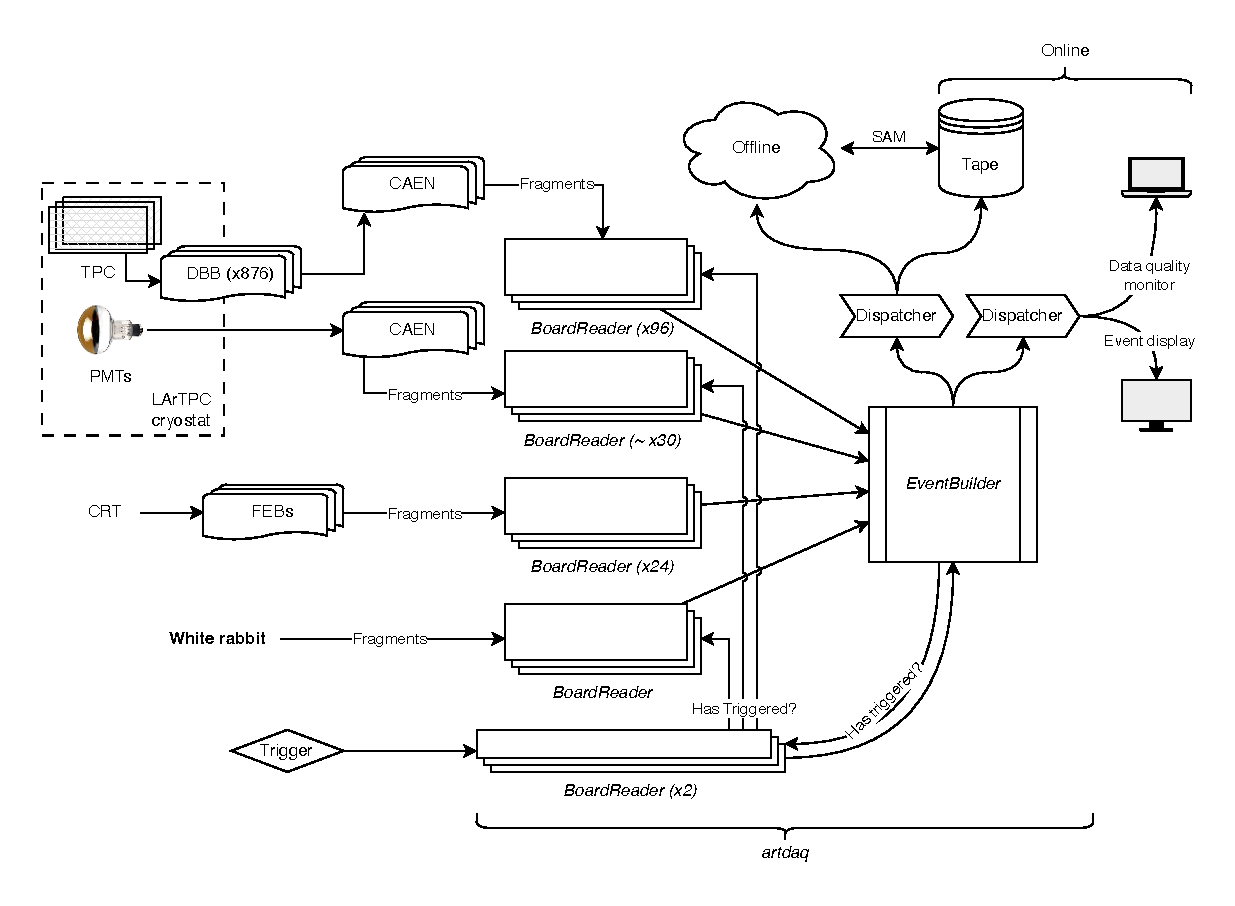
\includegraphics[width=\linewidth]{detector/DAQ_simplified.pdf}
    \caption[ICARUS DAQ illustration]{Simplified illustration of the ICARUS DAQ system. Further information is found in \autoref{sec:DAQ}. The number of parallel \emph{EventBuilder} instances could be defined $\geq1$, to allow for faster processing.}
    \label{fig:DAQ}
\end{figure}

\paragraph{TPC data} The TPC data input to the DAQ EventBuilder corresponds to the digitised waveforms from each TPC readout channel, representing the charge signal (as a function of time) induced by the motion of ionisation electrons drifted by the electric field inside the detector. 

\paragraph{PMT data} Similarly to the TPC data, the data from the PMTs correspond to the digitised waveforms of the readout of every PMT inside the detector. For any event triggered in coincidence with the beam spill, the digitised signals of all 360 PMTs are recorded in \SI{26}{\us} long time intervals, sampled at \SI{500}{\mega\hertz}. In addition to this data, whenever an off-time cosmic ray event crosses the volume, triggering scintillation light acquired by the PMTs in the \SI{+-1}{\ms} around the beam gate, all 180 PMTs belonging to the T300 module containing the interaction are recorded in \SI{10}{\us} long time intervals. 

\paragraph{CRT data} For the CRT system the DAQ acquisition and processing is slightly different \cite{ICARUS:2025rdw,Poppi:2023zmp,Poppi:2022vhg}. The ICARUS CRT components operate in self-trigger mode \cite{arteroponsStudyReconstructionNuMuCC, ICARUS:2025rdw}, whenever a CRT SiPM exceeds the threshold, the data from all 32 SiPM channels for each FEB is stored in internal buffers, holding up to \qtyrange{40}{80}{\ms} depending on which CRT sub-part is considered. The data from the top, bottom and side CRTs, which is a count as a function of time of photons readout by the SiPM at the ends of the scintillating strips, is aggregated within \SI{10}{\us} data fragments in the BoardReaders instances; once the global trigger is activated, \SI{+-25}{\ms} of CRT data fragments are sent from the BoardReader to the EventBuilder instance. 

\paragraph{Saved data} Downstream of the DAQ interface, events are written using the \emph{art} event-processing framework \cite{greenArtFramework2012} also developed at Fermilab, on which the \emph{artdaq} SDK is built. This allows interoperability between the DAQ interface and the offline analysis, without the need to convert the events saved from the DAQ interface into a format compatible with the high-level offline analysis. \emph{art} files are essentially ROOT files \cite{rene_brun_2019_3895860} with custom data types stored in them. The data collected by the ICARUS DAQ system are written in different file streams based on their specific acquisition mode, including the beam source (if on-beam), the specific trigger configuration active and its specific setting.

After a period of intense tests and validation of the system, the DAQ system allowed stable acquisition of high data rates up to \SI{5}{\hertz}. This is, however, larger than the amount of data input foreseen for the system with both BNB and NuMI beams and with the majority-based trigger configuration: the data throughput corresponds to ${\sim}\SI{1}{\hertz}$.

% In order to handle the large volumes of data stored on tape, the Fermilab-based SAM (serial access to metadata) system is exploited. This system associates a set of metadata information with each data file using Python scripts. This metadata is useful in offline analysis to create large datasets of files, identifying whether the files contain raw or processed data, run configuration, run number and so on.

% \section{ICARUS data processing}

% The output data files contain the aggregated data coming from all the \emph{BoardReader} instances in an event. For the TPC,  For the CRT system the DAQ acquisition and processing is slightly different \cite{ICARUS:2025rdw,Poppi:2023zmp,Poppi:2022vhg}. The ICARUS CRT components operate in self-trigger mode \cite{arteroponsStudyReconstructionNuMuCC, ICARUS:2025rdw}, whenever a CRT SiPM exceeds the threshold, the data from all 32 SiPM channels for each FEB is stored in internal buffers, holding up to \qtyrange{40}{80}{\ms} depending on which CRT sub-part is considered. The data from the top, bottom and side CRTs, which is a count as a function of time of photons readout by the SiPM at the ends of the scintillating strips, is aggregated within \SI{10}{\us} data fragments in the \emph{BoardReader}s instances; once the global trigger is activated, \SI{+-25}{\ms} of CRT data fragments are sent from the \emph{BoardReader} to the \emph{EventBuilder} instance. 

\section{ICARUS Data processing}

The output of all ICARUS sub-detectors is common across LArTPC detectors, which might have different TPC geometry and light collection configurations but share the same underlying technology. The \emph{art}-based \emph{LArSoft} framework \cite{Church:2013hea,Snider:2017wjd,Pordes:2017BL} is the common software development kit providing software infrastructure and algorithms for processing the collected data, and additionally providing tools that enable the simulation of the physics events and the detectors response, as well as the downstream event reconstruction. 

LArSoft allows to process the data by applying different algorithm, called modules, to the data stored in the \emph{art}/ROOT files. The modules are steered by configuration files that allow a great degree of flexibility. 
% The key to \emph{LArSoft} is the use of real-time configuration files that employ the \emph{Fermilab Hierarchical Configuration Language}, or \emph{FHiCL}, which specify how different modules of the processing chain should be run. 

The data processing and event reconstruction proceeds in two steps. First the raw data collected by the ICARUS DAQ is processed to produce a simpler representation of the signal, so from the raw digitized waveforms, \emph{hits} objects are created. Hits are objects containing the same information as the raw waveform, but in a more manegeable format. Inside this step, the signal on the wires, the signal from the PMTs and from the CRTs is analysed and translated into different hit types, depending on the subsystem. This step is commonly referred to as \emph{Stage0}. Once the data is processed, a second stage, referred to as \emph{Stage1}, aims at building a complete picture of the physics interaction happening inside the detector. This encompass, for example, the creation of the reconstructed interaction and its indetification from the hits reconstructed from the TPC wires. 

% When an event is saved from DAQ to data files and stored to tape, it is then available to be processed. The ICARUS data processing chain is split, like for many other LArTPC detectors, into two \emph{stages}, usually named \emph{Stage0} or \emph{reco1} and \emph{Stage1} or \emph{reco2}. Processing the raw collected data is a mandatory step in order for it to be properly analysed. 

% In the \emph{Stage0/reco1} step, all data  from the three sub-detectors is processed to produce a ``simpler'' description of the raw signal. This means to decode the raw signal and translate it into objects in the \emph{LArSoft} format for offline reconstruction. It also performs signal processing of the waveforms to identify physical signals, hits, that can then be used as input to the higher-level event reconstruction tools implemented in the \emph{Stage1/reco2} steps. 

\begin{figure}
    \centering
    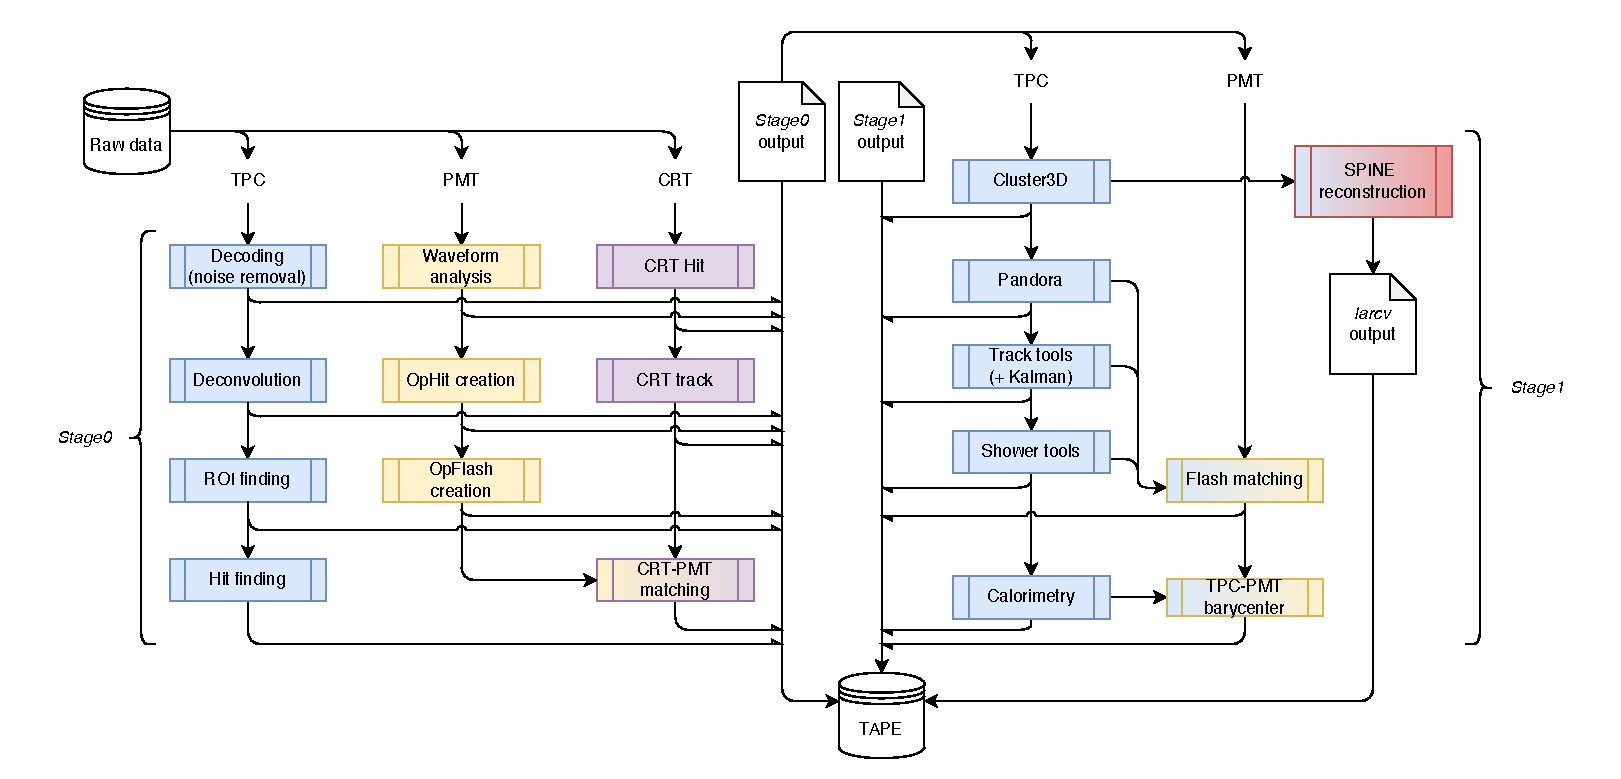
\includegraphics[width=\linewidth]{detector/data_processing_pipeline.pdf}
    \caption[\emph{Stage0} and \emph{Stage1} data processing pipeline]{Illustration of the data processing pipeline used in the ICARUS detector showing the steps involved in both \emph{Stage0} and \emph{Stage1}. }
    \label{fig:reco_stages}
\end{figure}

\autoref{fig:reco_stages} pictures the overall \emph{Stage0/Stage1} chain which is applied to the data files produced by the ICARUS DAQ. A detailed description of these steps follows in the next paragraphs. 

\subsection{Light reconstruction}

One of the first steps in \emph{Stage0} reconstruction addresses the reconstruction of the light signal. Reconstruction of the light signal associated with the event of interest is based on the recorded PMT signals in the events.

Light reconstruction starts from the identification of the PMT signal, using a threshold-based approach. To do so, a ``pedestal'' is defined, step which is performed using a sliding window, and mediating the photo electron counts to define the central value. The pedestal is subtracted from the raw signal, and the pedestal-subtracted waveform is used to identify the signal over the threshold, using three thresholds defining the start, tail and end time points of the PMT hit, called \emph{OpHit}. Once the three time values are identified, to OpHit is created. In a OpHit the start, end and tail timestamps are saved, and the area under the curve between these three points is computed. The integral of the waveform is proportional to the integral collected charge of the PMT that is protortional to the the collected light. If a start threshold is reached before the end of a previoud \emph{OpHit} the hit is truncated. \autoref{fig:PMT_reco}a shows the example of a PMT with a clear single \emph{OpHit}. 

After individual optical hits are reconstructed, they are clustered together into higher-level objects, called \emph{OpFlashes}, corresponding to multiple optical hits happening in proximity inside the detector, likely belonging to the same physical event inside the volume. \autoref{fig:PMT_reco}b shows the signal from multiple PMTs whose \emph{OpHit} will be clustered into a single \emph{OpFlash}.

All data products created in the \emph{Stage0} PMT processing are saved using the same \emph{LArSoft}-based structure to ROOT files. 

\begin{figure}
    \centering
    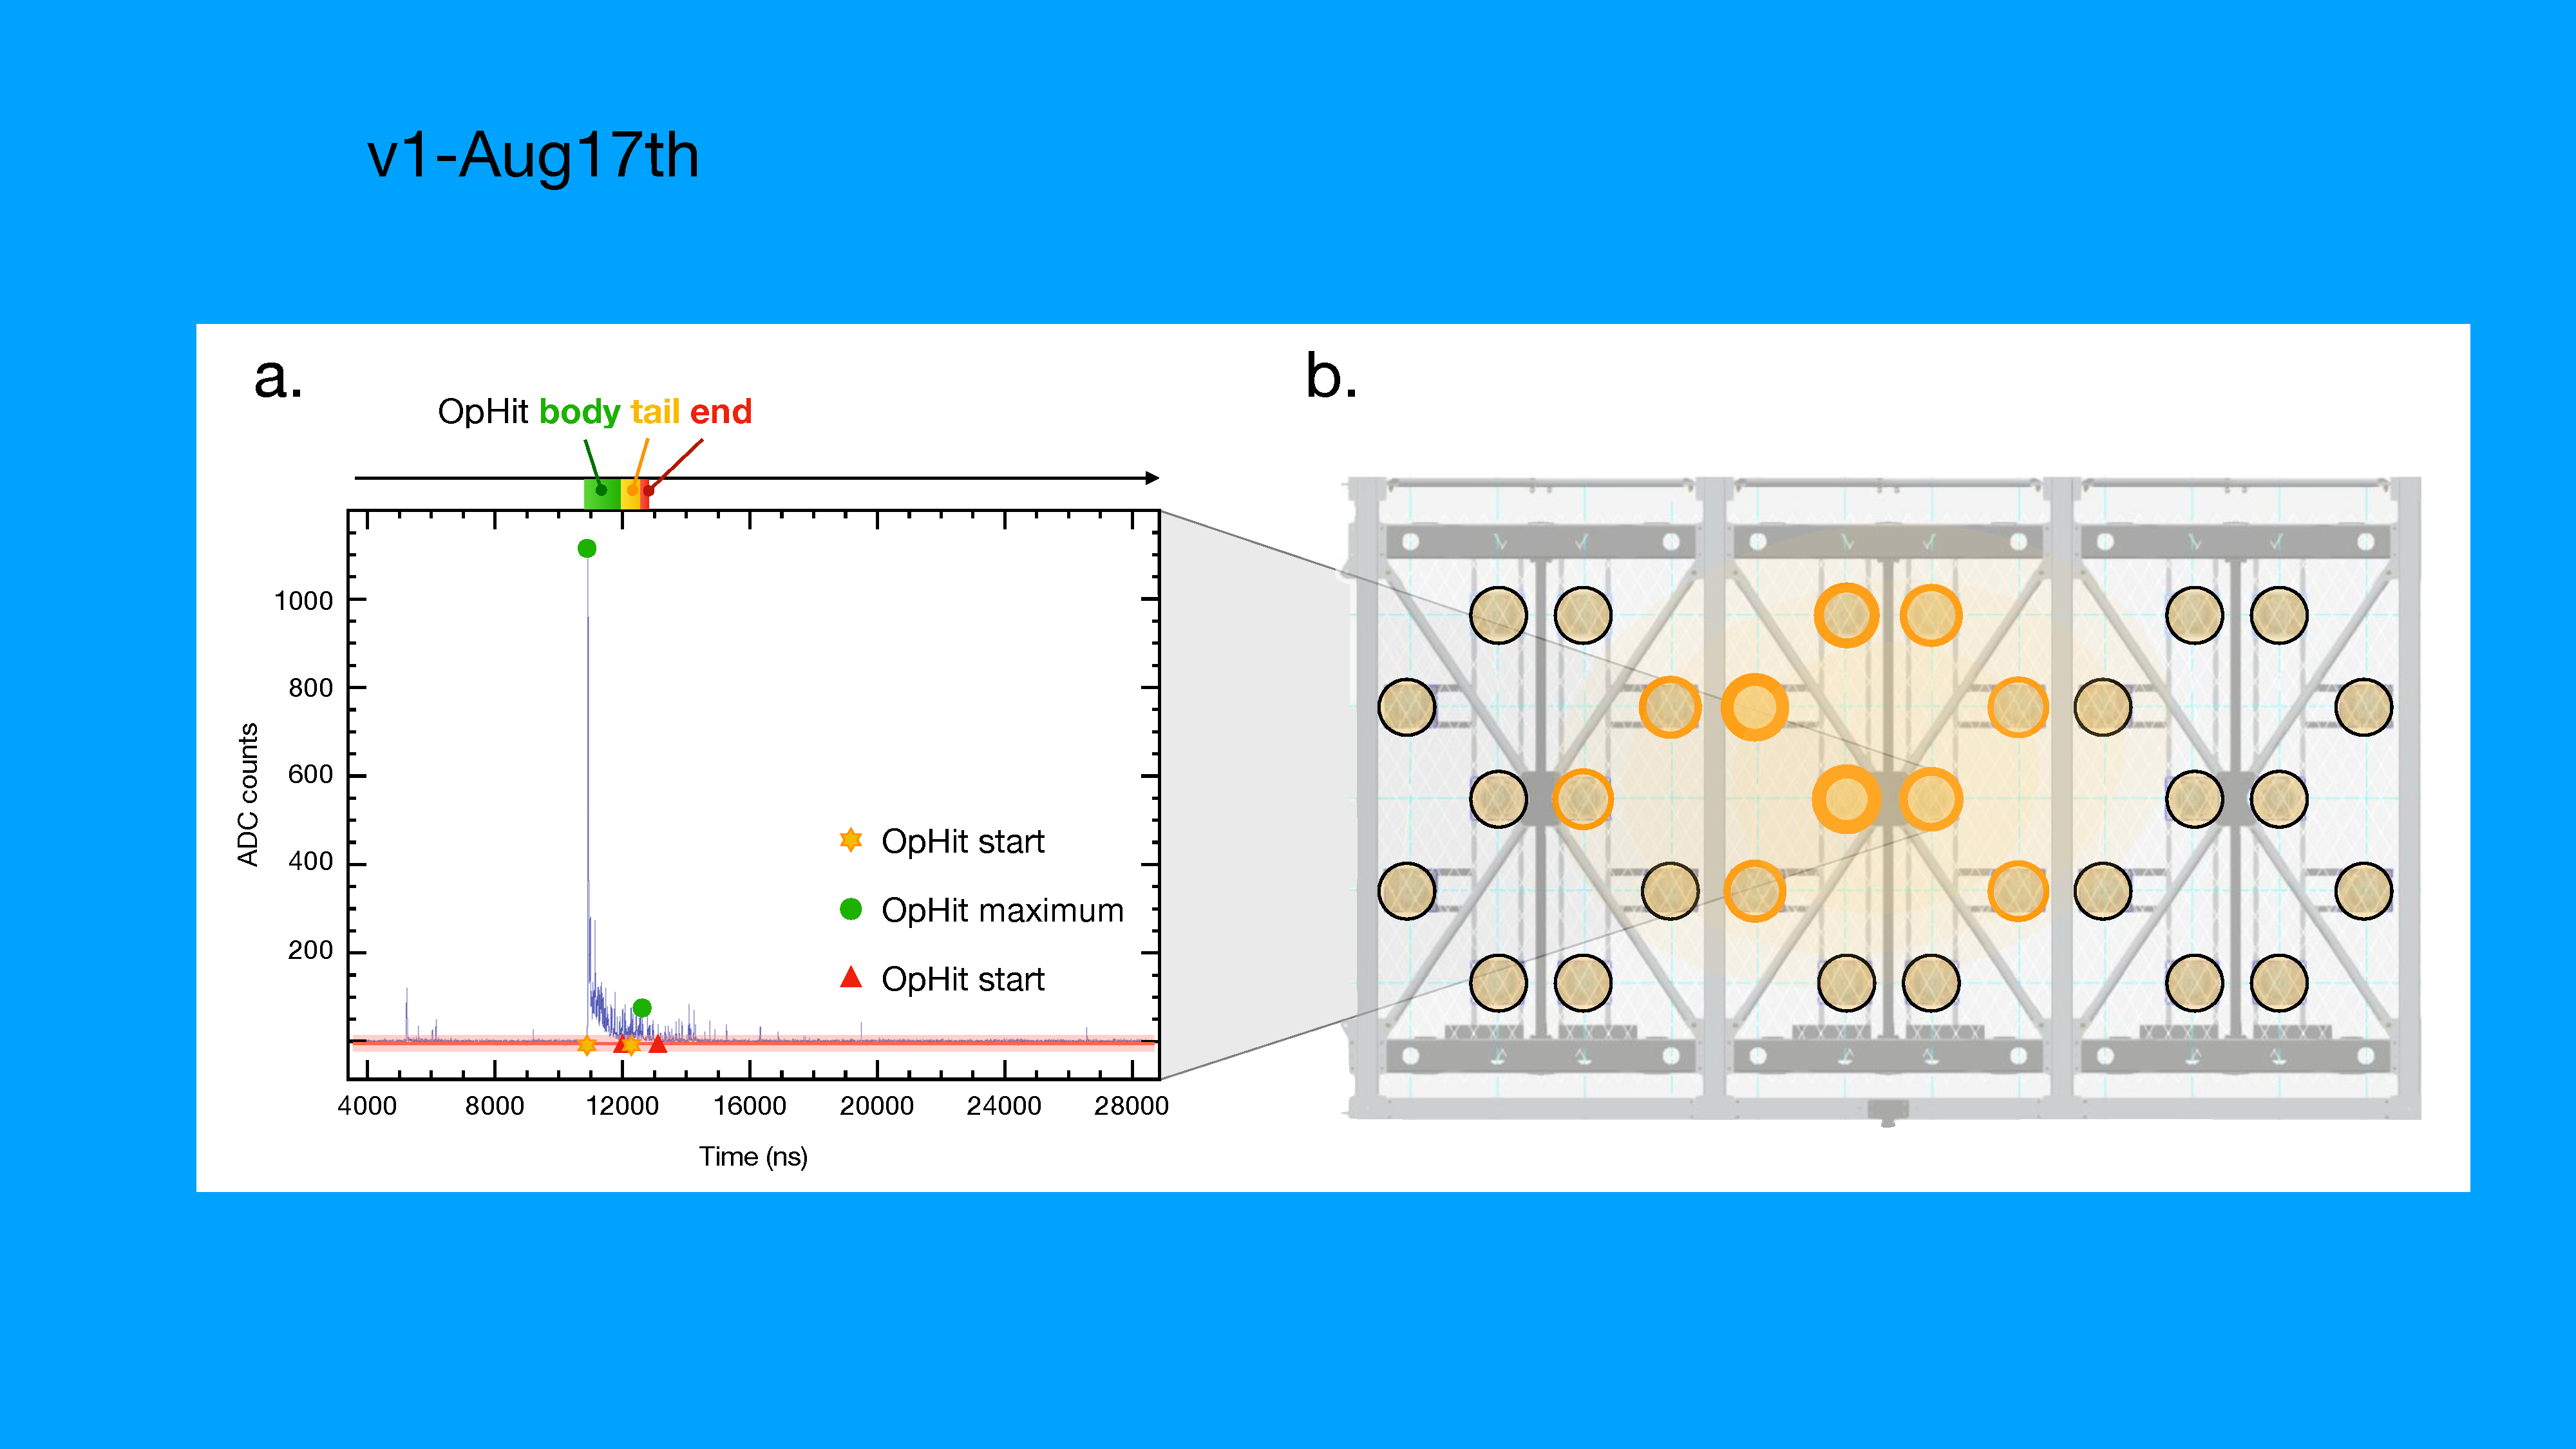
\includegraphics[width=\linewidth,trim={5.5cm 7cm 3.5cm 9cm},clip]{detector/PMT_reco.pdf}
    \caption[PMT reconstructed \emph{OpHits}]{Illustration of an interaction as seen by the PMTs inside the detector volume. (a) shows the pedestal-subtracted waveform produced by a single fired PMT, where the \emph{OpHit} information is marked on top, with the three regions (body, tail and end) highlighted. (b) shows all the PMTs activated during an event in the TPC volume; the PMTs collecting a light signal above the defined threshold are indicated in yellow. Their signal is used to build the so called \emph{OpFlash} object.}
    \label{fig:PMT_reco}
\end{figure}

\subsection{Cosmic ray tagger reconstruction} 

The first step in the reconstruction of the CRT signal is the extraction of the number of photoelectrons $n_\mathrm{p.e.}$. This is done starting from the raw ADC counts, subtracting the pedestal and correcting for the amplification gain \begin{equation}
    n_\mathrm{p.e.} = \frac{\mathrm{\#ADC} - \mathrm{ped}}{G}. 
\end{equation} 

A preliminary selection for the side CRT data is performed, requiring each signal to be above a \SI{7.5}{pe} threshold. Top CRT data are instead selected with a different requirement, i.e. a ``quadruple'' signal coincidence is necessary to generate a hit as shown in \autoref{fig:CRT_reco}a. At this point it is possible to create the CRT \emph{Hit} objects for side and top CRTs. Two timestamps are associated to each hit: $T_0$ identifying the global timing of the recorded hit and provided by the White Rabbit switch system, and $T_1$ which identifies the relative timing of the hit with respect to the trigger. Additionally each CRT hit object has its position in the detector reference frame associated. Due to the differences in the CRT modules between side and top CRT, the position computation is slightly different. 

\begin{figure}
    \centering
    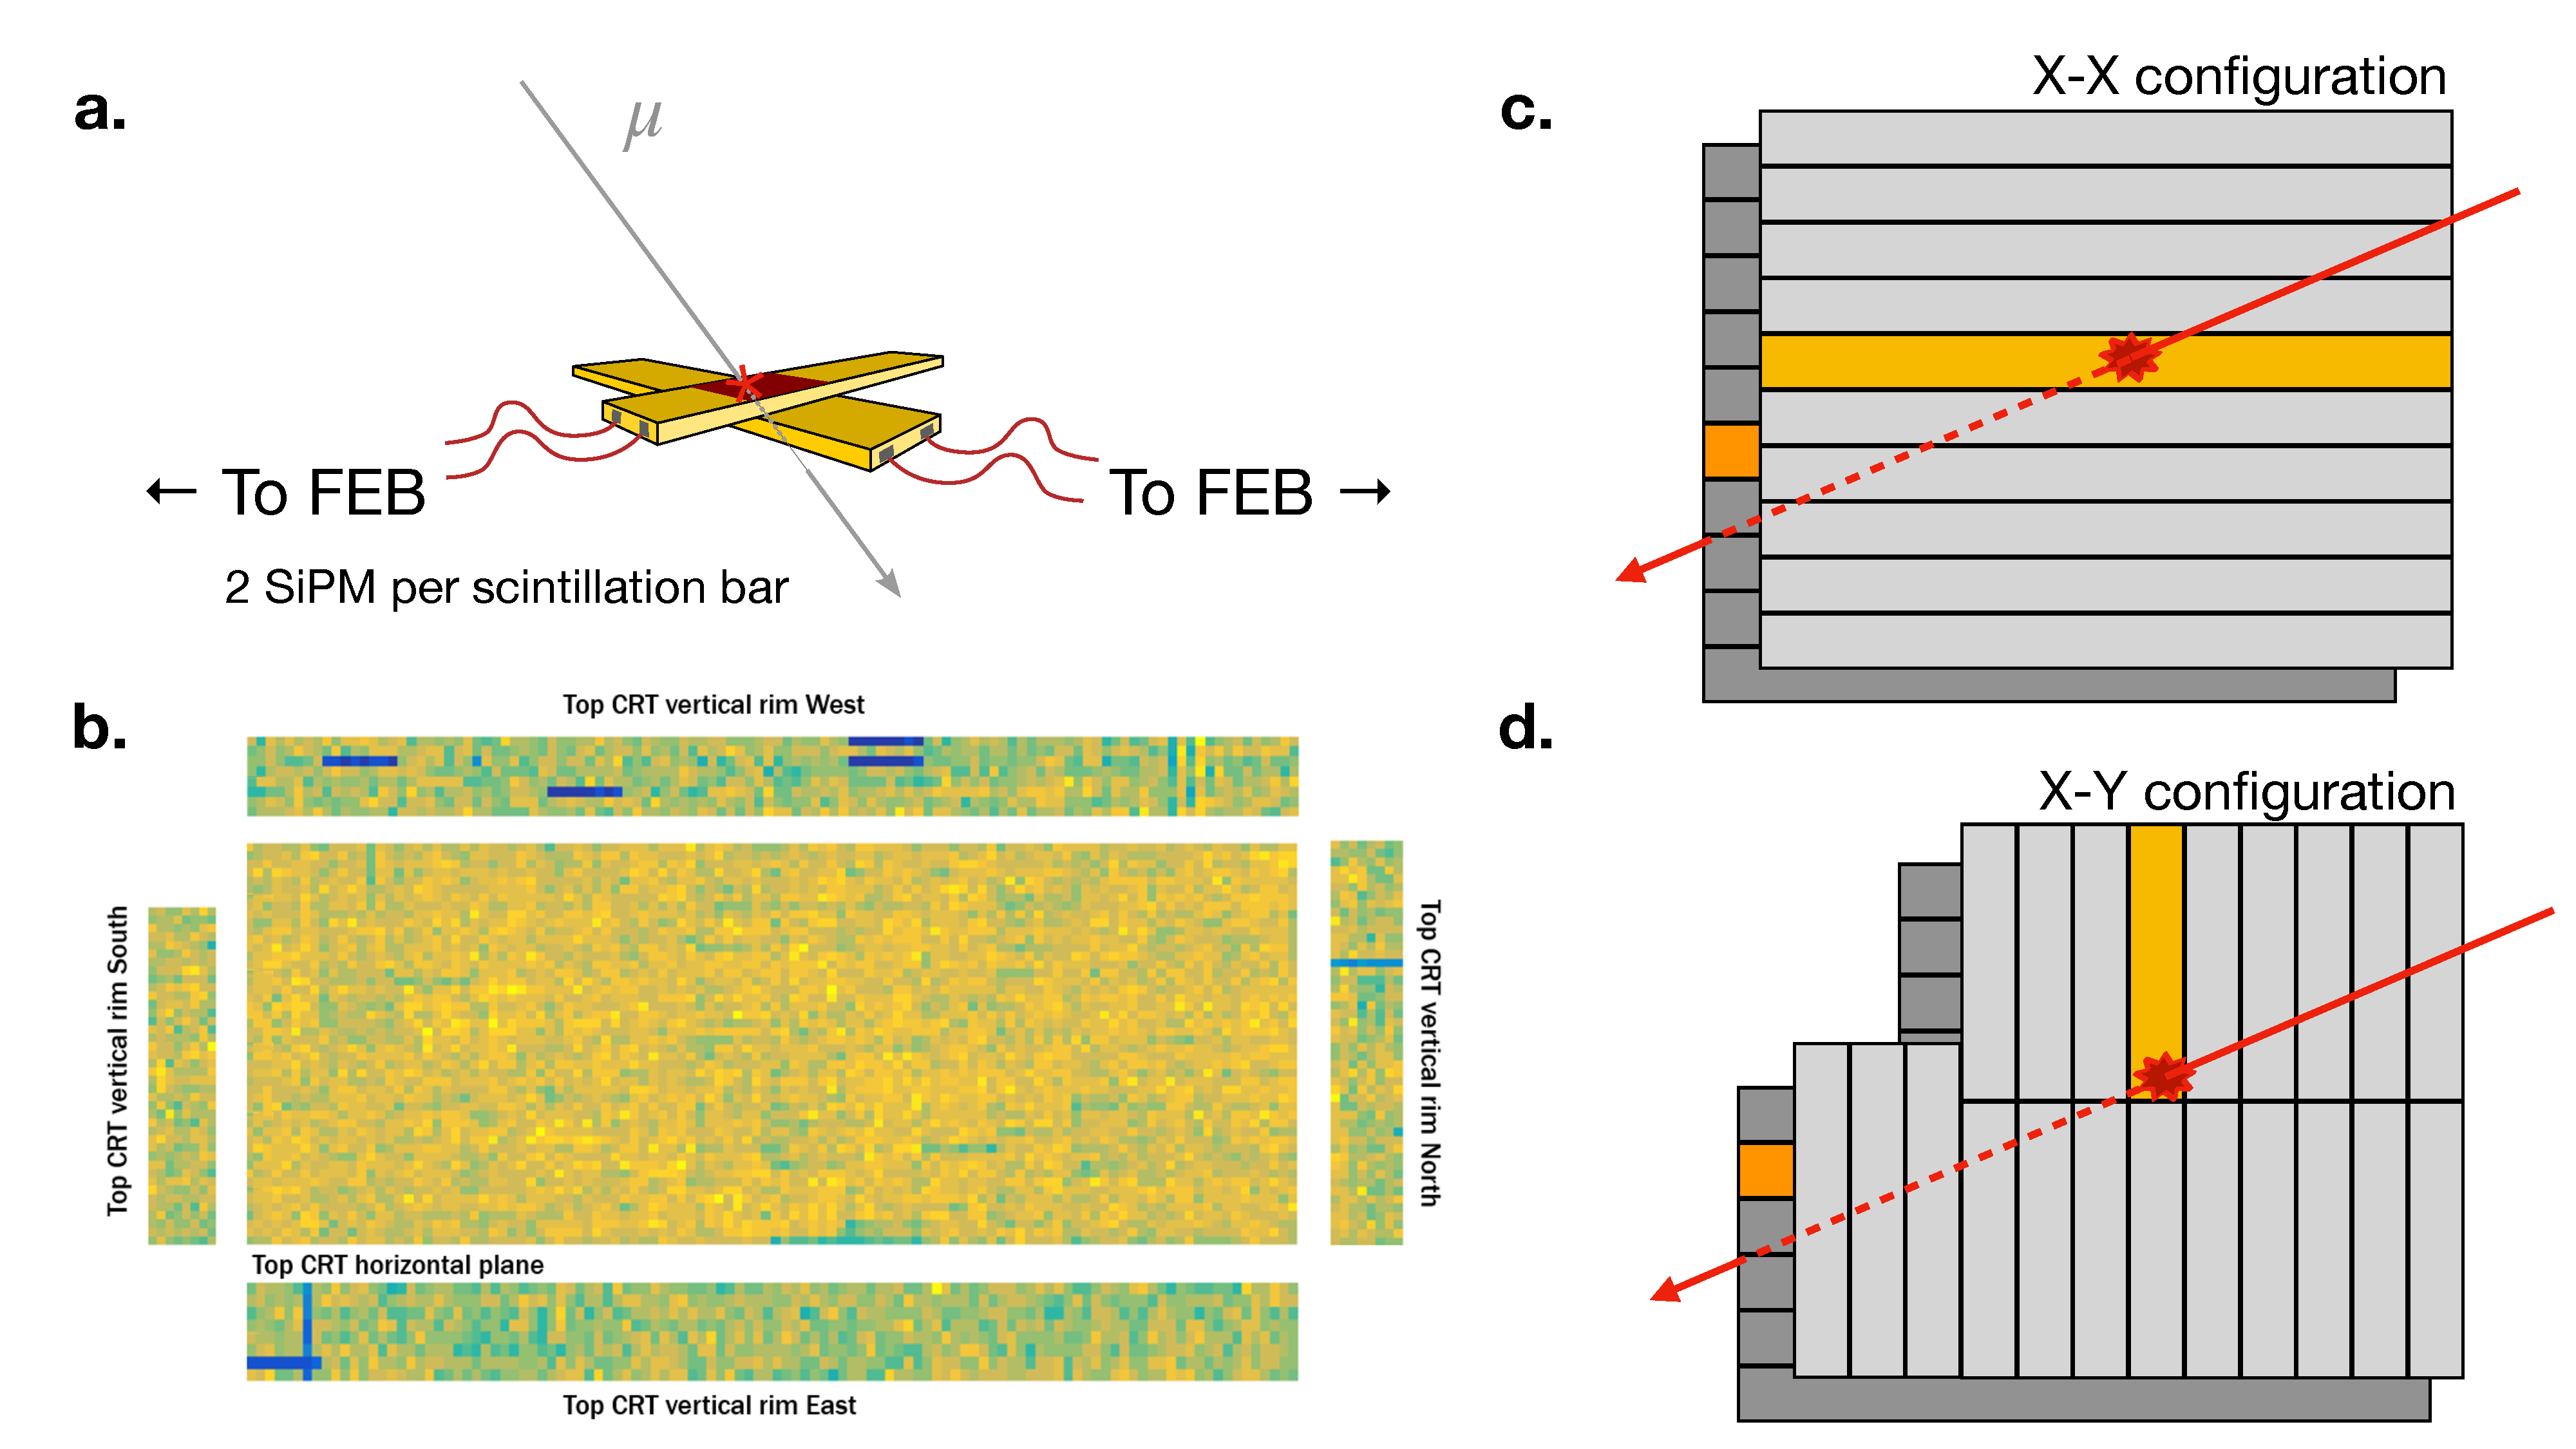
\includegraphics[width=\linewidth]{detector/CRT_all.pdf}
    \caption[CRT Hit reconstruction in space]{Illustration of CRT hit position reconstruction. (a) shows the reconstruction for the top CRT modules, where the coincidence between two scintillation bars is required. (b) shows the distribution of the CRT hits reconstructed in the different regions of the Top CRT. Blue regions correspond to malfunctioning channels. (c) and (d) show respectively the configuration fo the east/west and north side CRT, and south CRT modules. (b) is taken from \cite{Poppi:2023zmp}, (a), (c) and (d) are adapted from \cite{arteroponsStudyReconstructionNuMuCC}.}
    \label{fig:CRT_reco}
\end{figure}

By using the quadruple coincidence, the position of top CRT hits in each module is known with a granularity of \qtyproduct[product-units=power]{23x23}{\cm}. \autoref{fig:CRT_reco}b shows the distribution of the CRT hits using a collected calibration run. 

For the side CRT modules the position in the detector (reference) frame is reconstructed with a slightly different approach. The coincidence of adjacent layers is reconstructed offline via software because the same modules are being read by multiple FEBs. Hit scintillator strips are identified by selecting in each FEB the channel that generated the FEB trigger signal, which is the one with the highest charge amplitude. \autoref{fig:CRT_reco}c and d show two of the configurations of the CRT side module strips. The triggering strip is shown in yellow, and the red star shows the interaction point. The north, east and west side CRTs have the X-X configuration shown in \autoref{fig:CRT_reco}c. For these components, if two opposite SiPM signals are collected within \SI{150}{\ns}, and read out by two FEBs, the longitudinal position (across the strip) can be computed with respect to the centre position of the strip by comparing the $T_0$ timestamps recorded by each FEB:     \begin{equation}
    z = \qty(T_B - T_A)/2 \cdot v_\mathrm{wls}, 
\end{equation} where $T_A$ and $T_B$ are, respectively, the two timestamps recorded by the FEBs  and $v_\mathrm{wls}$ is the group velocity of the light signal inside the wavelength shifter fibre. The south CRT wall instead was built with the X-Y configuration shown in \autoref{fig:CRT_reco}d. In this case, a coincidence offline software-based approach similar to that used for the top CRT component is employed, by exploiting the orthogonal relative position of the outer and the inner strips. 

The last step performed in \emph{Stage0} concerns the temporal matching of the light and CRT information. This step is crucial, especially for higher-level processing, where it can be exploited to improve the efficiency by which correct interactions are selected inside the detector, rejecting out-of-time activity using the CRT-PMT match. 

\subsection{Wireplanes signal reconstruction}

The wire data is the waveform readout of the \num{53248} individual wires. The first step of the wire signal processing happens online directly on the readout cards installed in the TPC online computers, and aims at removing the coherent noise from the wires \cite{MicroBooNE:2017qiu}. Only minimal further processing is performed online, which leaves more scope for reprocessing the raw data using improved signal processing tools. The recorded waveforms are in ADC count/tick units, where the amplitude of the signal is expressed in ADC counts and the time information in ticks, each corresponding to \SI{0.4}{\us} in the ICARUS TPC timing. \autoref{fig:TPC_signal} shows a sample of the data collected by the three planes, exhibiting the characteristic bipolar shape for the two induction wire planes and a unipolar signal for the collection plane. 

\begin{figure}
    \centering
    \subfloat[]{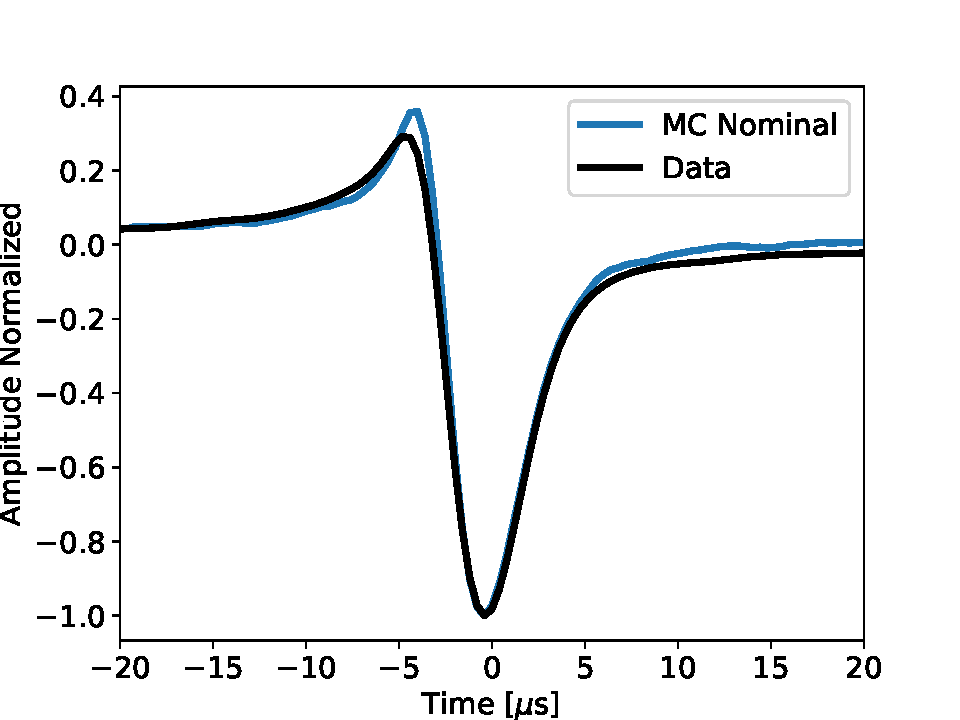
\includegraphics[width=0.3\linewidth]{detector/wvf_data_MCNominal_a20_P0.pdf}\label{fig:TPC_wire_i1}}
    \subfloat[]{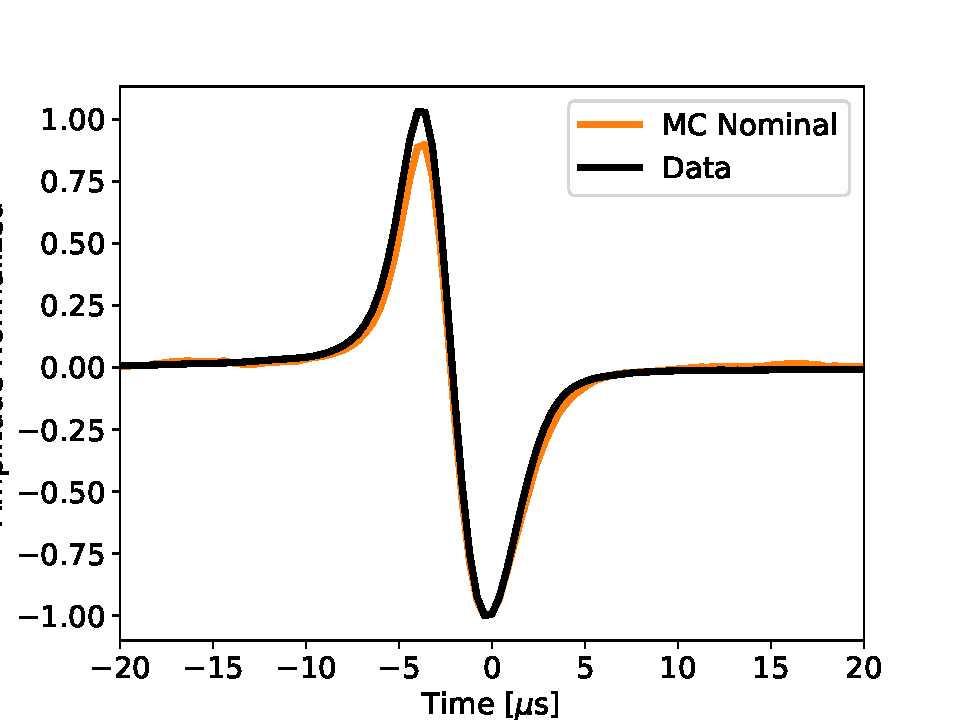
\includegraphics[width=0.3\linewidth]{detector/wvf_data_MCNominal_a20_P1.pdf}\label{fig:TPC_wire_i2}}
    \subfloat[]{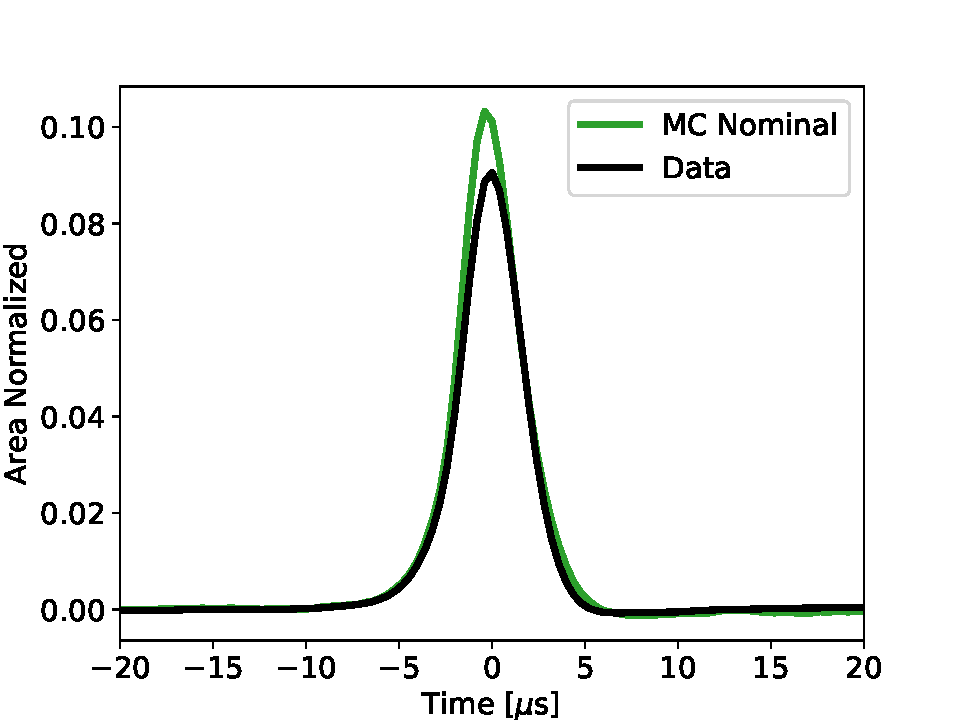
\includegraphics[width=0.3\linewidth]{detector/wvf_data_MCNominal_a20_P2.pdf}\label{fig:TPC_wire_c}}
    \caption[TPC plane signal]{Typical \emph{raw} signal captured by the three planes (induction-1 \ref{sub@fig:TPC_wire_i1}, induction-2 \ref{sub@fig:TPC_wire_i2} and collection \ref{sub@fig:TPC_wire_c}) showing the characteristic bipolar signal for the two induction plane and the unipolar shape for the collection plane. The signal is averaged in the $\theta_{xw}$ angle, where $x$ is the drift coordinate, and $w$ is the orientation of the wires in the $w$ plane. Picture taken from \cite{ICARUS:2024hmk}. }
    \label{fig:TPC_signal}
\end{figure}

In order to deconvolve the TPC wire signal from the deformation induced on the true signal by the electric field effects and shaping effects coming from the front end electronic, three major steps are addressed in \emph{Stage0}: \begin{inparaenum}
    \item the wire signals are deconvolved from the TPC electronic response functions, so that all three wire signal are also unipolar in shape;
    \item the signal is analysed in order to define the region-of-interest (ROI) with a threshold-based algorithm; 
    \item each ROI is finally fit using a Gaussian function, whose area is proportional to the number of drift electrons generating the signal. 
\end{inparaenum} Given the relevance of these steps of the processing chains, we will briefly describe them in the next paragraphs.

\paragraph{Wire signal deconvolution} The wire signal shape can provide information on the deposited charge of drift electrons and subsequently of the depositd enrgy of the particle interactiong in LAr. However, in order to explain such dependency, the effects related to the distorsion of the true signal, due to the drifting electric field and the electronic response, must be deconvolved from the readout signal. The readout signal $R(t)$ on the wires can be expressed as the convolution of serial effects of signal formation, electron propagation, electrostatic field response around the wires and processing by the DAQ to the true electronic signal, so that each wire channel response function can be factorised as \begin{equation}
    \begin{aligned}
        R(t, t')&=\mathrm{Ionization\ \otimes\ Recombination\ \otimes\ Diffusion\ and\ Attachment\ \otimes} \\
        &\quad \quad \quad \mathrm{Field\ response\ \otimes\ Electronic\ response\ \otimes\ Electronic\ noise}
    \end{aligned} 
\end{equation} In order to recover the desired ionisation electron yield, useful to measure the deposited energy per wire inside the detector as a function of time, it is necessary to unfold these effects. 

The ICARUS experiment exploits a signal processing chain similar to other LArTPC experiments, performing a deconvolution in time of the signal waveforms. Ideally, after the deconvolution step, the signal pulse produced by a charged track on the wire would be Gaussian-shaped, with an integral area proportional to the deposited charge, i.e. a proxy of the energy, inside LAr. The signal recorded on the wires is the convolution of the response function $R$ with the ``true'' $S$ signal, \begin{equation}
    M(t') = \int_{-\infty}^{+\infty} R(t,t')\ S(t)\ \dd t;
\end{equation} Using the properties of the Fourier transforms, this can be written in the frequency domain as $\mathcal M(\omega) = \mathcal R(\omega)\cdot \mathcal S(\omega)$, which can be inverted to extract the true wire signal $\mathcal S(\omega)$. This approach, referred to as ``one-dimensional'' deconvolution, is currently employed in most of LArTPC detectors. However, this assumes that the charge distribution on each wire is independent from the charge distribution on the wires in its vicinity. However, as shown in \cite{MicroBooNE:2018swd,MicroBooNE:2018vro}, it was demonstrated that this is not always true. Furthermore, while in general accounting for this effect implies small additional corrections to the overall deposited charge there are cases where wire channel correlations are non negligible. For example, for isochronous tracks (i.e. tracks lying parallel to the wires, which is frequent for the induction-1 wires given the specific ICARUS geometry), nearby wire channels correlation effects can create destructive interference patterns.

\begin{figure}
    \centering
    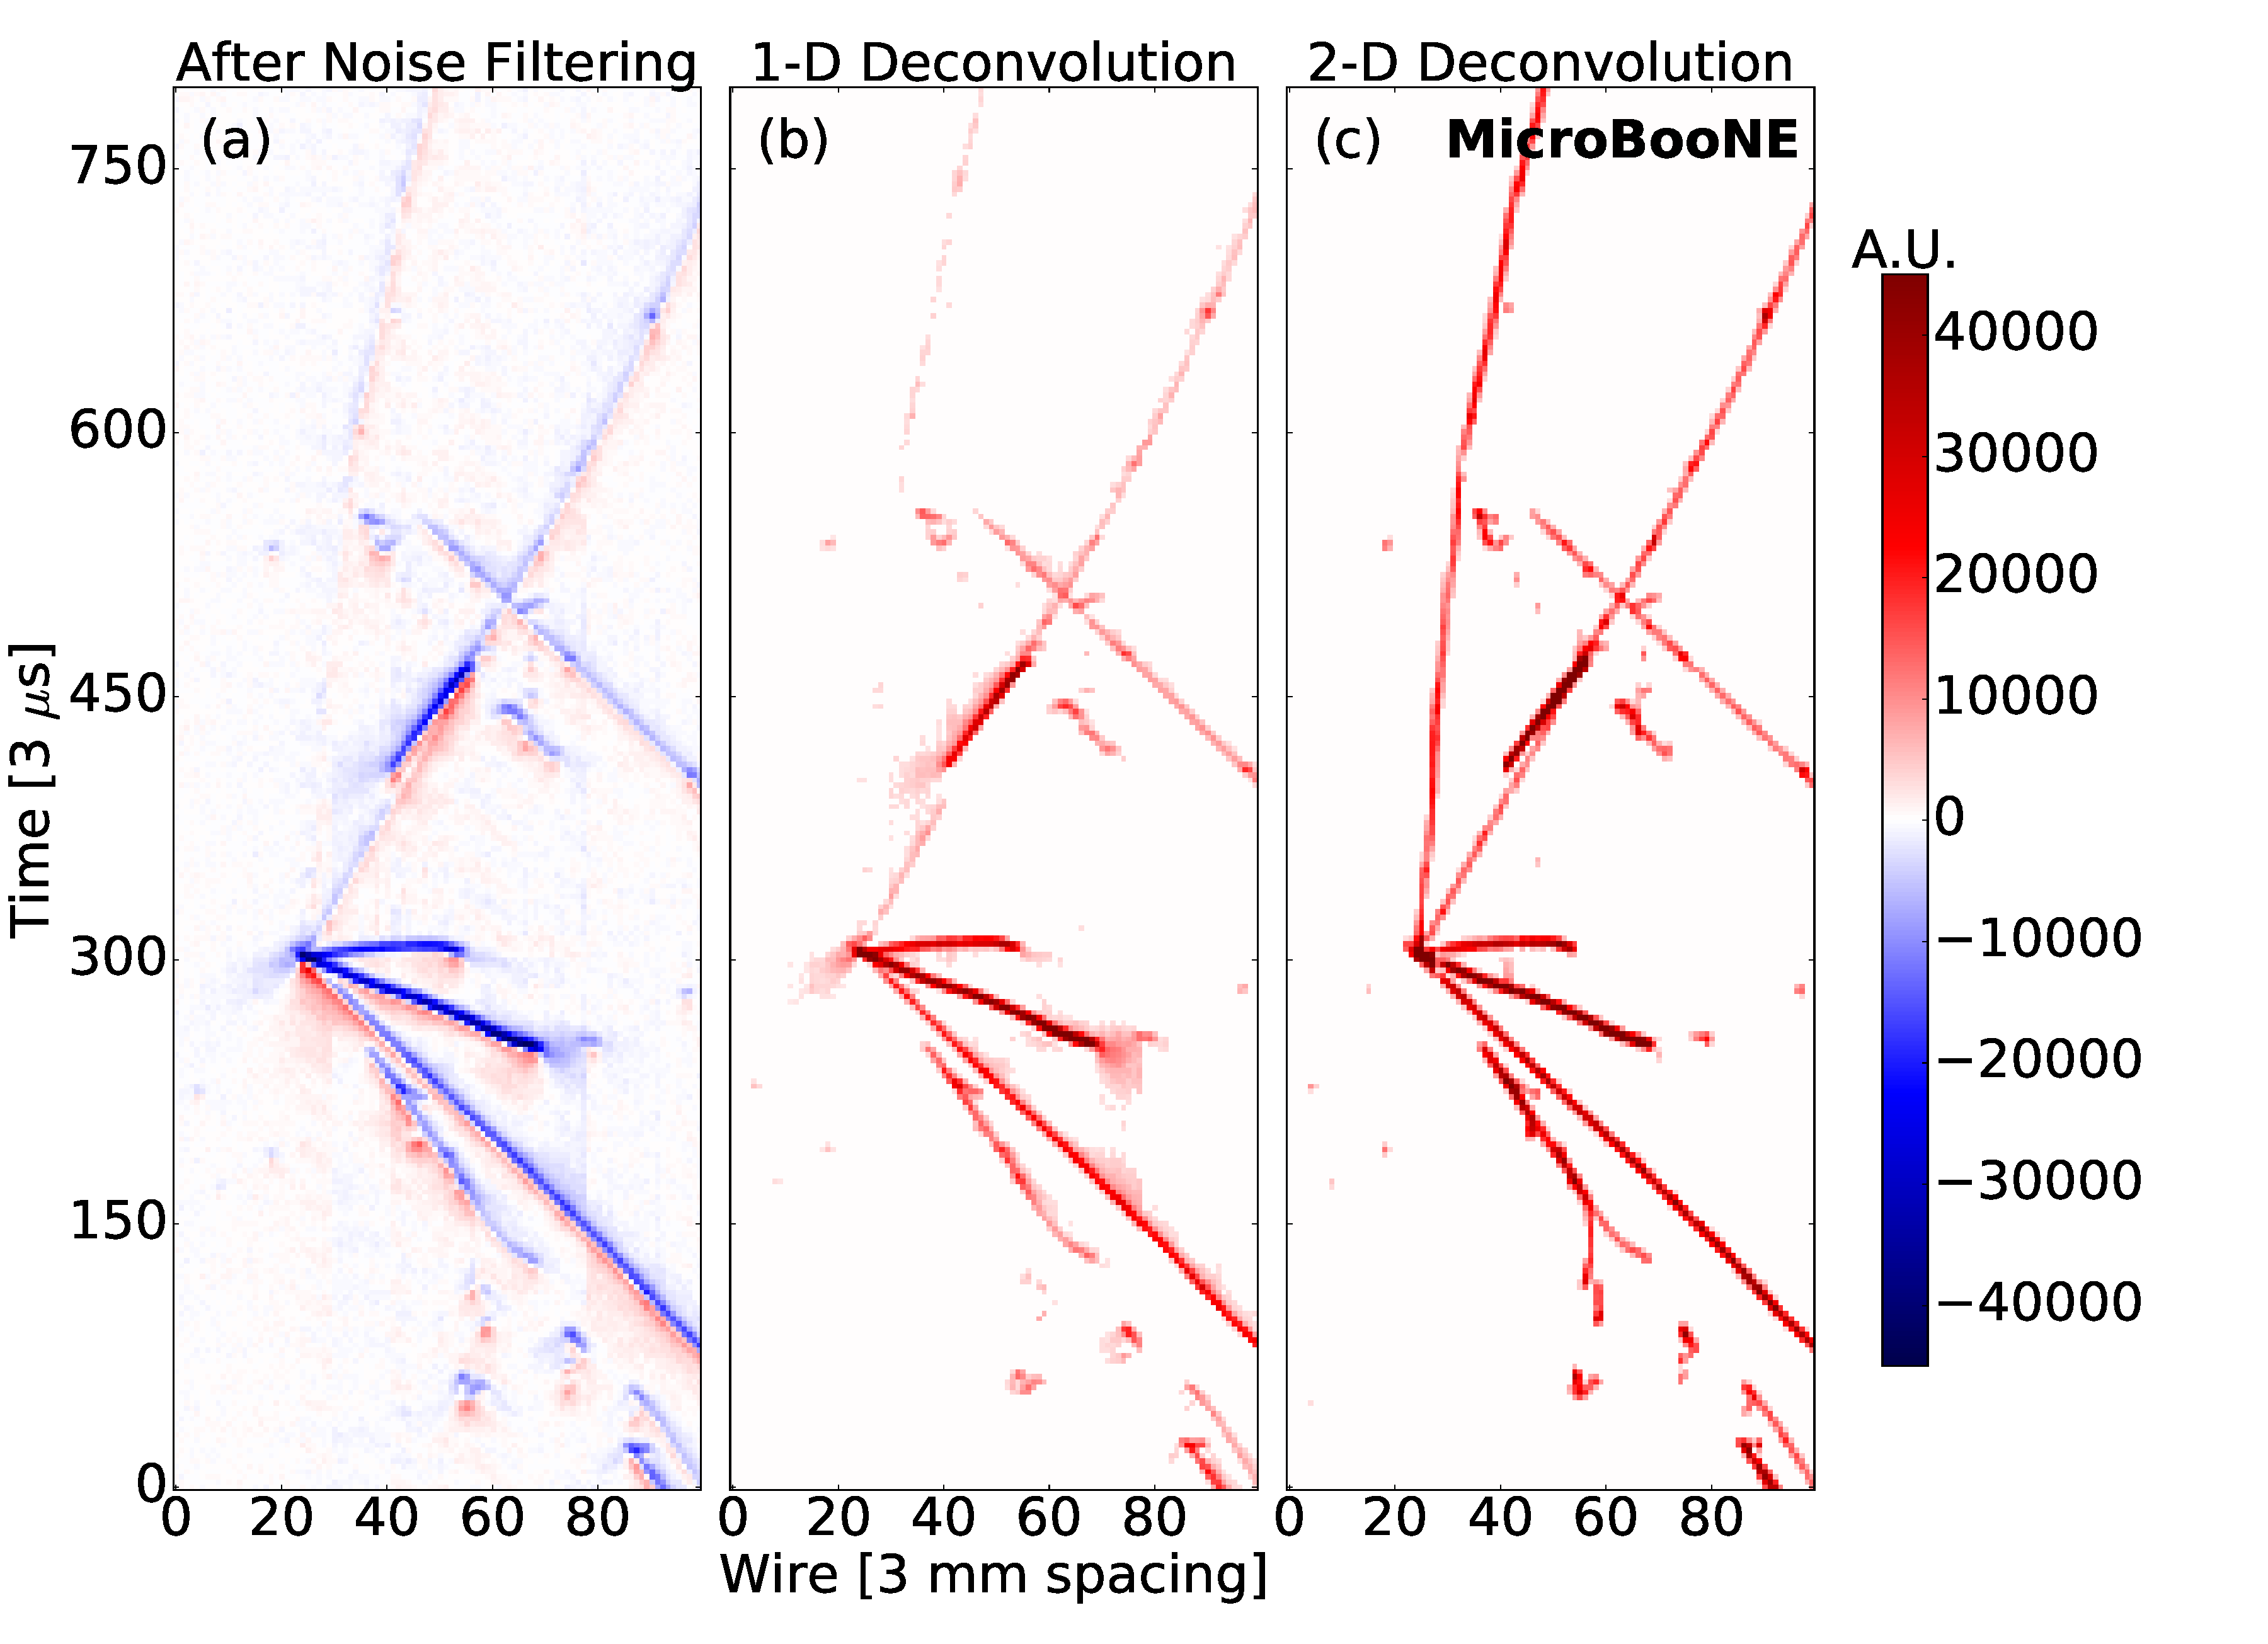
\includegraphics[width=0.85\linewidth]{detector/noiseVs1DVs2D.pdf}
    \caption[TPC signal processing]{Example of the effect of signal processing using the one-dimensional deconvolution approach employed in ICARUS (b) with respect to the noise-filtered data (a). Figure (c) shows the same event using a two-dimensional deconvolution approach, i.e. performing the deconvolution both in the time direction as well as in the direction of the wires. Picture taken from \cite{MicroBooNE:2018swd}. }
    \label{fig:uBooNE_signalProc}
\end{figure}

In \cite{MicroBooNE:2018swd,MicroBooNE:2018vro} a solution to this issue is presented: it consists in the application of two-dimensional deconvolution techniques where both time and wire channel are taken into account. This provides a strong and computationally efficient method to better extract the distribution of ionisation electrons. \autoref{fig:uBooNE_signalProc} shows the result of the 1D and 2D approaches as tested by the MicroBooNE experiment. Efforts aimed at adapting two-dimensional deconvolution techniques to ICARUS TPC raw data and testing their impact on the reconstruction performance are currently ongoing. Preliminary results indicate a remarkable enhancement in reconstruction efficiency specifically for track-like particle trajectories.

\paragraph{ROI finding} After the deconvolution, we need to identify interesting regions of the TPC wire signals as function of time. With a threshold-based algorithm we find the interesting regions (ROIs) to look for the signal hits, i.e. segments of waveform corresponding to the signal. ROIs can be actually relevant to iteratively improve the performances of the 1D/2D deconvolution steps, by minimising the time-domain region over which the deconvolution is performed. Once ROIs are identified, a baseline ADC counts value can be assigned to all the remaining times in the waveform, thereby drastically reducing the size of these data products inside the data files. 

\paragraph{Gaussian \emph{Hit} creation} Upon the identification of ROIs, the final step is the creation of the \emph{Hit}s objects. A \emph{Hit} is a two-dimensional object representing a cluster of electric drift charges, arriving at a certain time on a certain wire. The hit-finding algorithm runs under the assumption the distribution of the drift charges is Gaussian. Operating on the deconvolved ROI segments of the waveforms, it tries to fit one or multiple Gaussian distributions onto the signal shape. The parameters derived from the Gaussian fit are properties of the hits and include the area under the Gaussian(s), mean and FWHM of the distribution and its multiplicity. The area corresponds to the cumulative charge deposited by the electrons and proportional to the deposited energy inside the detector; the mean and the FWHM represent the hit peak time and its width. 

At this point, a collection of 2D hits for each plane of wires is available. For each reconstructed event, the three 2D views of the planes are stored and used as input for the event reconstruction taking place inside \emph{Stage1}. 

\section{TPC event reconstruction} \label{sec:TPC_reco_gen}

\emph{Stage1} is dedicated to performing the high-level event reconstruction, taking the \emph{Hit} objects created by the modules of \emph{Stage0} and transforming them to build the full interaction picture. This part of the event reconstruction interests primarily the information extracted from TPC and PMT sub-detectors, since it is expected for most neutrino interactions (${\sim}\SI{80}{\percent}$) to be contained inside the LAr volume, hence not expected to generate a CRT signal. 

To perform the event reconstruction inside the TPC, the starting point is given by the three collections of 2D hits created in \emph{Stage0}.

The hit-finding algorithm, providing the collections of 2D hits, is optimised to prefer efficiency over purity, reaching an efficiency greater than \SI{99}{\percent}; this might, however, lead to the creation of non-physical hits, especially in very noisy regions, that might cause failures in the pattern recognition steps. To prevent such problems, the collection of 2D hits produced by the hitfinding algorithm are filtered using the \emph{Cluster3D} algorithm. This preliminary step of the \emph{Stage1} reconstruction runs over the set of wires of the three planes and, exploiting the common $x$ drift coordinate, looks for time-correlated hits across the three planes. If matches are not found, or hits are isolated, then they are filtered out. The resulting filtered collection of hits is used as the input for the subsequent high-level reconstruction tools that are, in the contex of the ICARUS experiment, the Pandora topological reconstruction \cite{MicroBooNE:2017xvs} and the SPINE machine-learning-based recontruction \cite{Drielsma:2021jdv}. 

% This thesis focuses on developing tools for the event reconstruction process briefly described below, which is referred to as ``Pandora event reconstruction'' within the collaboration. However, recent inroads in Computer Vision (CV) and Machine Learning (ML) have motivated a new approach to the analysis of particle imaging detector data. Additionally, having multiple different approaches to event reconstruction can be crucial in proving the robustness of each one. 

% This thesis is mostly geared toward the Pandora event reconstruction, of which an in-depth description is provided in \autoref{sec:Pandora} and subsequent sections. In \autoref{sec:SPINE} is also provided a description of the SPINE reconstruction framework. 

Pandora has been the baseline for the event reconstruction within the SBN program since its first days. The Pandora reconstruction chain takes the three 2D hits produced by the hit-finding algorithm as input, filtered by the cluster3D tool, performing a topological reconstruction of the tracks and showers taking part in the interaction to allow a hiearchical reconstruction of the neutrino candidate events. It specifically promotes the idea of a multi-algorithm approach to solving pattern-recognition problems. In this approach, the input building blocks (hits) describing the pattern recognition problem are considered by large numbers of decoupled algorithms. Each algorithm targets a specific event topology and controls operations such as collecting hits together in clusters, merging or splitting clusters, or collecting clusters in order to build a representation of reconstructed particles in the detector. The algorithms gradually build up a picture of the underlying events and collectively provide a robust reconstruction. % Further details are provided in \autoref{sec:Pandora}. 


Recent inroads in Computer Vision (CV) and Machine Learning (ML) have motivated a new approach to the analysis of particle imaging detector data, and efforts within the ICARUS collaboration have been made to develop a machinel-learning-based approach to the event recosntruction. SPINE (Scalable Particle Identification with Neural Embeddings) project serve this purpose. Unlike the Pandora reconstruction, which starts from the 2D colection of hits on the readout planes, the SPINE reconstruction leverage a fully three-dimensional reconstruction starting from the 3D space points created by the cluster3D algorithm. This way ambiguities that might arise in the Pandora reconstruction are resolved. However, this approach introduces other difficulties, as will be addressed in dedicated paragraphs. 

This thesis has the aim of performing a detailed validation study of the Pandora-based event reconstruction, and so a more detailed descritpion is given in the sections following \autoref{sec:Pandora}. The SPINE approach to the event reconstruction is briefly presented and discussed in \autoref{sec:SPINE}.

\subsection{Geometry of the ICARUS detector}

The Pandora reconstruction --- as any reconstruction paradigm for LArTPC would do --- heavily exploits the geometrical characteristic of the detector. Newer LArTPC detectors employ a common geometry to make it effortless to transition the software codebase from one to another. Being the first of its kind and since its original physical scope extended beyond that of the SBN program, the ICARUS detector TPC geometry is unique. As already mentioned in \autoref{sec:ICARUS_T600}, and illustrated in \autoref{fig:i2_c_planes_wirepitch_detail}, ICARUS wire planes have some peculiarities. First, the wire orientation is different from other LArTPCs currently in use for neutrino experiments, including SBND and ProtoDUNE: for reasons related both to mechanical constraints and topological reconstruction, it is customary to build TPC wire planes with wires oriented \SI{+-60}{\degree} with respect to the vertical direction for the first two induction planes ($u$/$v$), and have the collection ($w$) plane wires vertical, whereas in the ICARUS detector the first induction plane features horizontal wires, and the second induction and collection planes are oriented \SI{+-60}{\degree} with respect to the horizontal. The reason for the horizontal wires was dictated by the target physics analyses for the ICARUS experiment at LNGS, especially for the detection of cosmic-induced particles. Due to mechanical limitations, however, it was not possible to have \SI{18}{\metre} long wires kept at the tension needed for the detector operation, so they had to be split into two 9-meter-long sections. 

The geometrical parameter that is core for the Pandora software when performing the 3D reconstruction of the wire planes 2D projections is the angle at which the wire planes are oriented. This information is used to perform the spatial reconstruction of the hits collected in the different planes, using projective geometry. In Pandora each plane is associated to a so called view and each view has associated the angle at which wires are oriented. In most LArTPCs the mapping between views and planes is univocal. For example, considering the SBND APA, both East and West APAs feature the $u$ plane at $+\SI{60}{\degree}$, the $v$ plane at $-\SI{60}{\degree}$ and the $w$ plane at \SI{0}{\degree} with respect to the vertical direction. In the ICARUS TPC, however, the requirement to have the induction-2 and collection plane's wire angle oriented in the same direction if seen in the drifting direction (see, for reference, \autoref{fig:i2_c_planes_wirepitch_detail}) means that the mapping is not unique and depends on which TPC of each T300 module is being considered. As the association between the readout plane and view is not guaranteed in the ICARUS geometry, except for the induction-1 plane, there are some caveats with the Pandora reconstruction. This is the case, for example, when the reconstruction assumes that the $w$ view is the collection plane. For some steps of the current reconstruction, this step has been addressed. 

\subsection{Pandora approach to the event reconstruction} \label{sec:Pandora}

As already anticipated, Pandora takes an innovative approach to the topological event reconstruction, splitting the problem of pattern recognition among the action of smaller, decoupled algorithms. The Pandora framework is embedded inside \emph{LArSoft} and accessed via the \emph{LArPandora} module, that handles the Pandora event reconstruction. The ICARUS detector consists of two separated T300 modules; thus, two parallel instances of the Pandora reconstruction are run on each event, corresponding to the east and west cryostats. Each Pandora instance runs the full list of algorithms on the corresponding T300 module. 

The inputs are the collections of 2D hits in the $x$--wire plane, with $x$ representing the drift time and the second coordinate being the wire number. The $x$ coordinate is common across the views and thus is exploited to match the hits from different planes. The output of the pattern recognition algorithms are the Particle Flow Particles, or PFParticles, objects; each PFParticle correspond to a distinct track or shower, and, through the action of subsequent algorithms, is associated to a list of 2D clusters, which are groups of hits on the same plane belonging to the same reconstructed object. Each PFParticle is also associated with a set of 3D positions (named SpacePoints) corresponding to the reconstructed 3D trajectory and with a vertex position, defining its interaction point or its first energy deposition. PFParticles are finally arranged in a hierarchy, which identifies parent-daughter relationships for a given interaction candidate. For each interaction defined as neutrino-like, one empty PFParticle is created, identifying the neutrino PFParticle, and thus associated with the primary interaction vertex. \autoref{fig:LArPandora_dependencies} shows all data products produced by Pandora and their interdependency. 

\begin{figure}
    \centering
    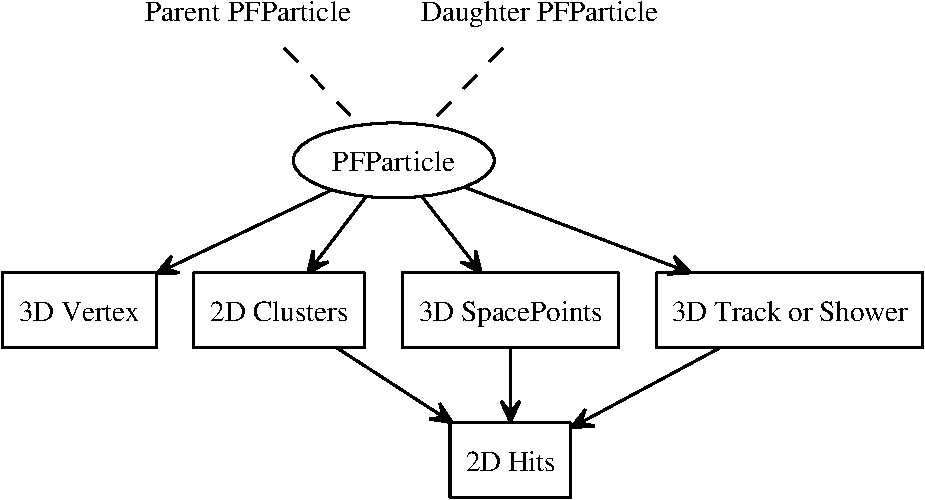
\includegraphics[width=0.75\linewidth]{pandora/LArSoftOutput.pdf}
    \caption[LArPandora output data products]{The Pandora output data products. Navigation along PFParticle hierarchies is achieved using the PFParticle interface, represented by dashed lines. Navigation from PFParticles to their associated objects is represented by solid arrows. Picture taken from \cite{MicroBooNE:2017xvs}. }
    \label{fig:LArPandora_dependencies}
\end{figure}

Three Pandora multi-algorithm reconstruction paths have been created for use in the analysis of ICARUS data: PandoraFastReco, PandoraCosmic and PandoraNeutrino. The last two are, as the names suggest, aimed at the reconstruction of precise interaction topologies; namely,  PandoraCosmic is optimised for the reconstruction of cosmic-ray muons and their daughter delta-rays, whereas PandoraNeutrino is optimised for the reconstruction of neutrino interactions. The PandoraFastReco path is run prior to both PandoraNeutrino and PandoraCosmic, with the precise aim of identifying and excluding from further processing steps \emph{unambiguous} cosmic-ray muons, employing a faster reconstruction pipeline. The output of the PandraFastReco path corresponds to a list of candidate cosmic rays. This list is then examined by a tagging module which identifies unambiguous cosmic-ray muons, based on their topological features, and removes their hits from the list. This enables an initial coarse separation of candidate signal events from background, thereby restricting the use of complex topological reconstruction algorithms to the most interesting events and reducing the overall computational cost of the reconstruction chain. \autoref{fig:pandora} illustrates the subsequent steps applied to each event by the Pandora reconstruction. 

\begin{sidewaysfigure}
    \centering
    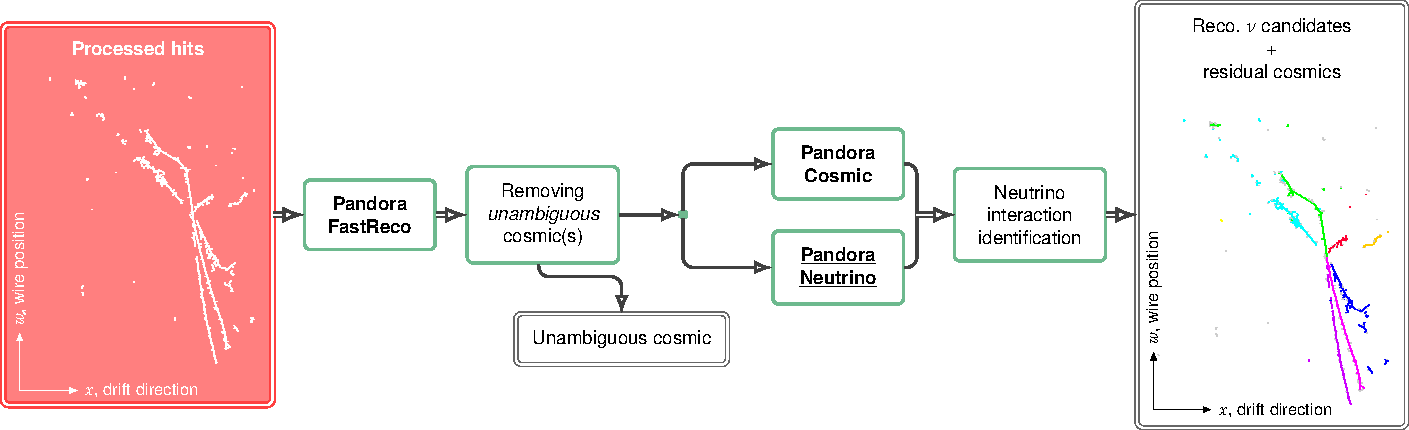
\includegraphics[width=\linewidth]{pandora/figure_Pandora/pandora.pdf}
    \caption[Overview of the Pandora reconstruction chain]{Illustration of the Pandora reconstruction chain. Starting from a set of image-like collections of 2D hits, as shown in the left red panel, the approach is to first address a fast and rough reconstruction, aimed at removing the particles that are clearly cosmic-ray muons. Then each interaction inside the detector is passed through both PandoraCosmic and PandoraNeutrino chains to refine its reconstruction. }
    \label{fig:pandora}
\end{sidewaysfigure}

\subsection{PandoraFastReco: \emph{unambiguous} cosmic hits removal} \label{sec:fast_reco}

The first Pandora reconstruction path applied to the events consists of a set of tools aimed at performing a coarse reconstruction of all the hits identified during the readout window. This way, long straight tracks coming from muons crossing the detector volume are identified. A list of ``unambiguous'' cosmic-ray particle is created, using a classification of these reconstructed objects on the basis of topological considerations. The PandoraFastReco step shares most of the algorithms with the PandoraCosmic reconstruction path, since the goal is similar and entails the reconstruction of interactions characterised by a long straight track, usually crossing the full detector volume. The path, illustrated in \autoref{fig:PandoraFastReco}, is composed of four main stages, that are the subject of the next paragraphs. 

\begin{figure}
    \centering
    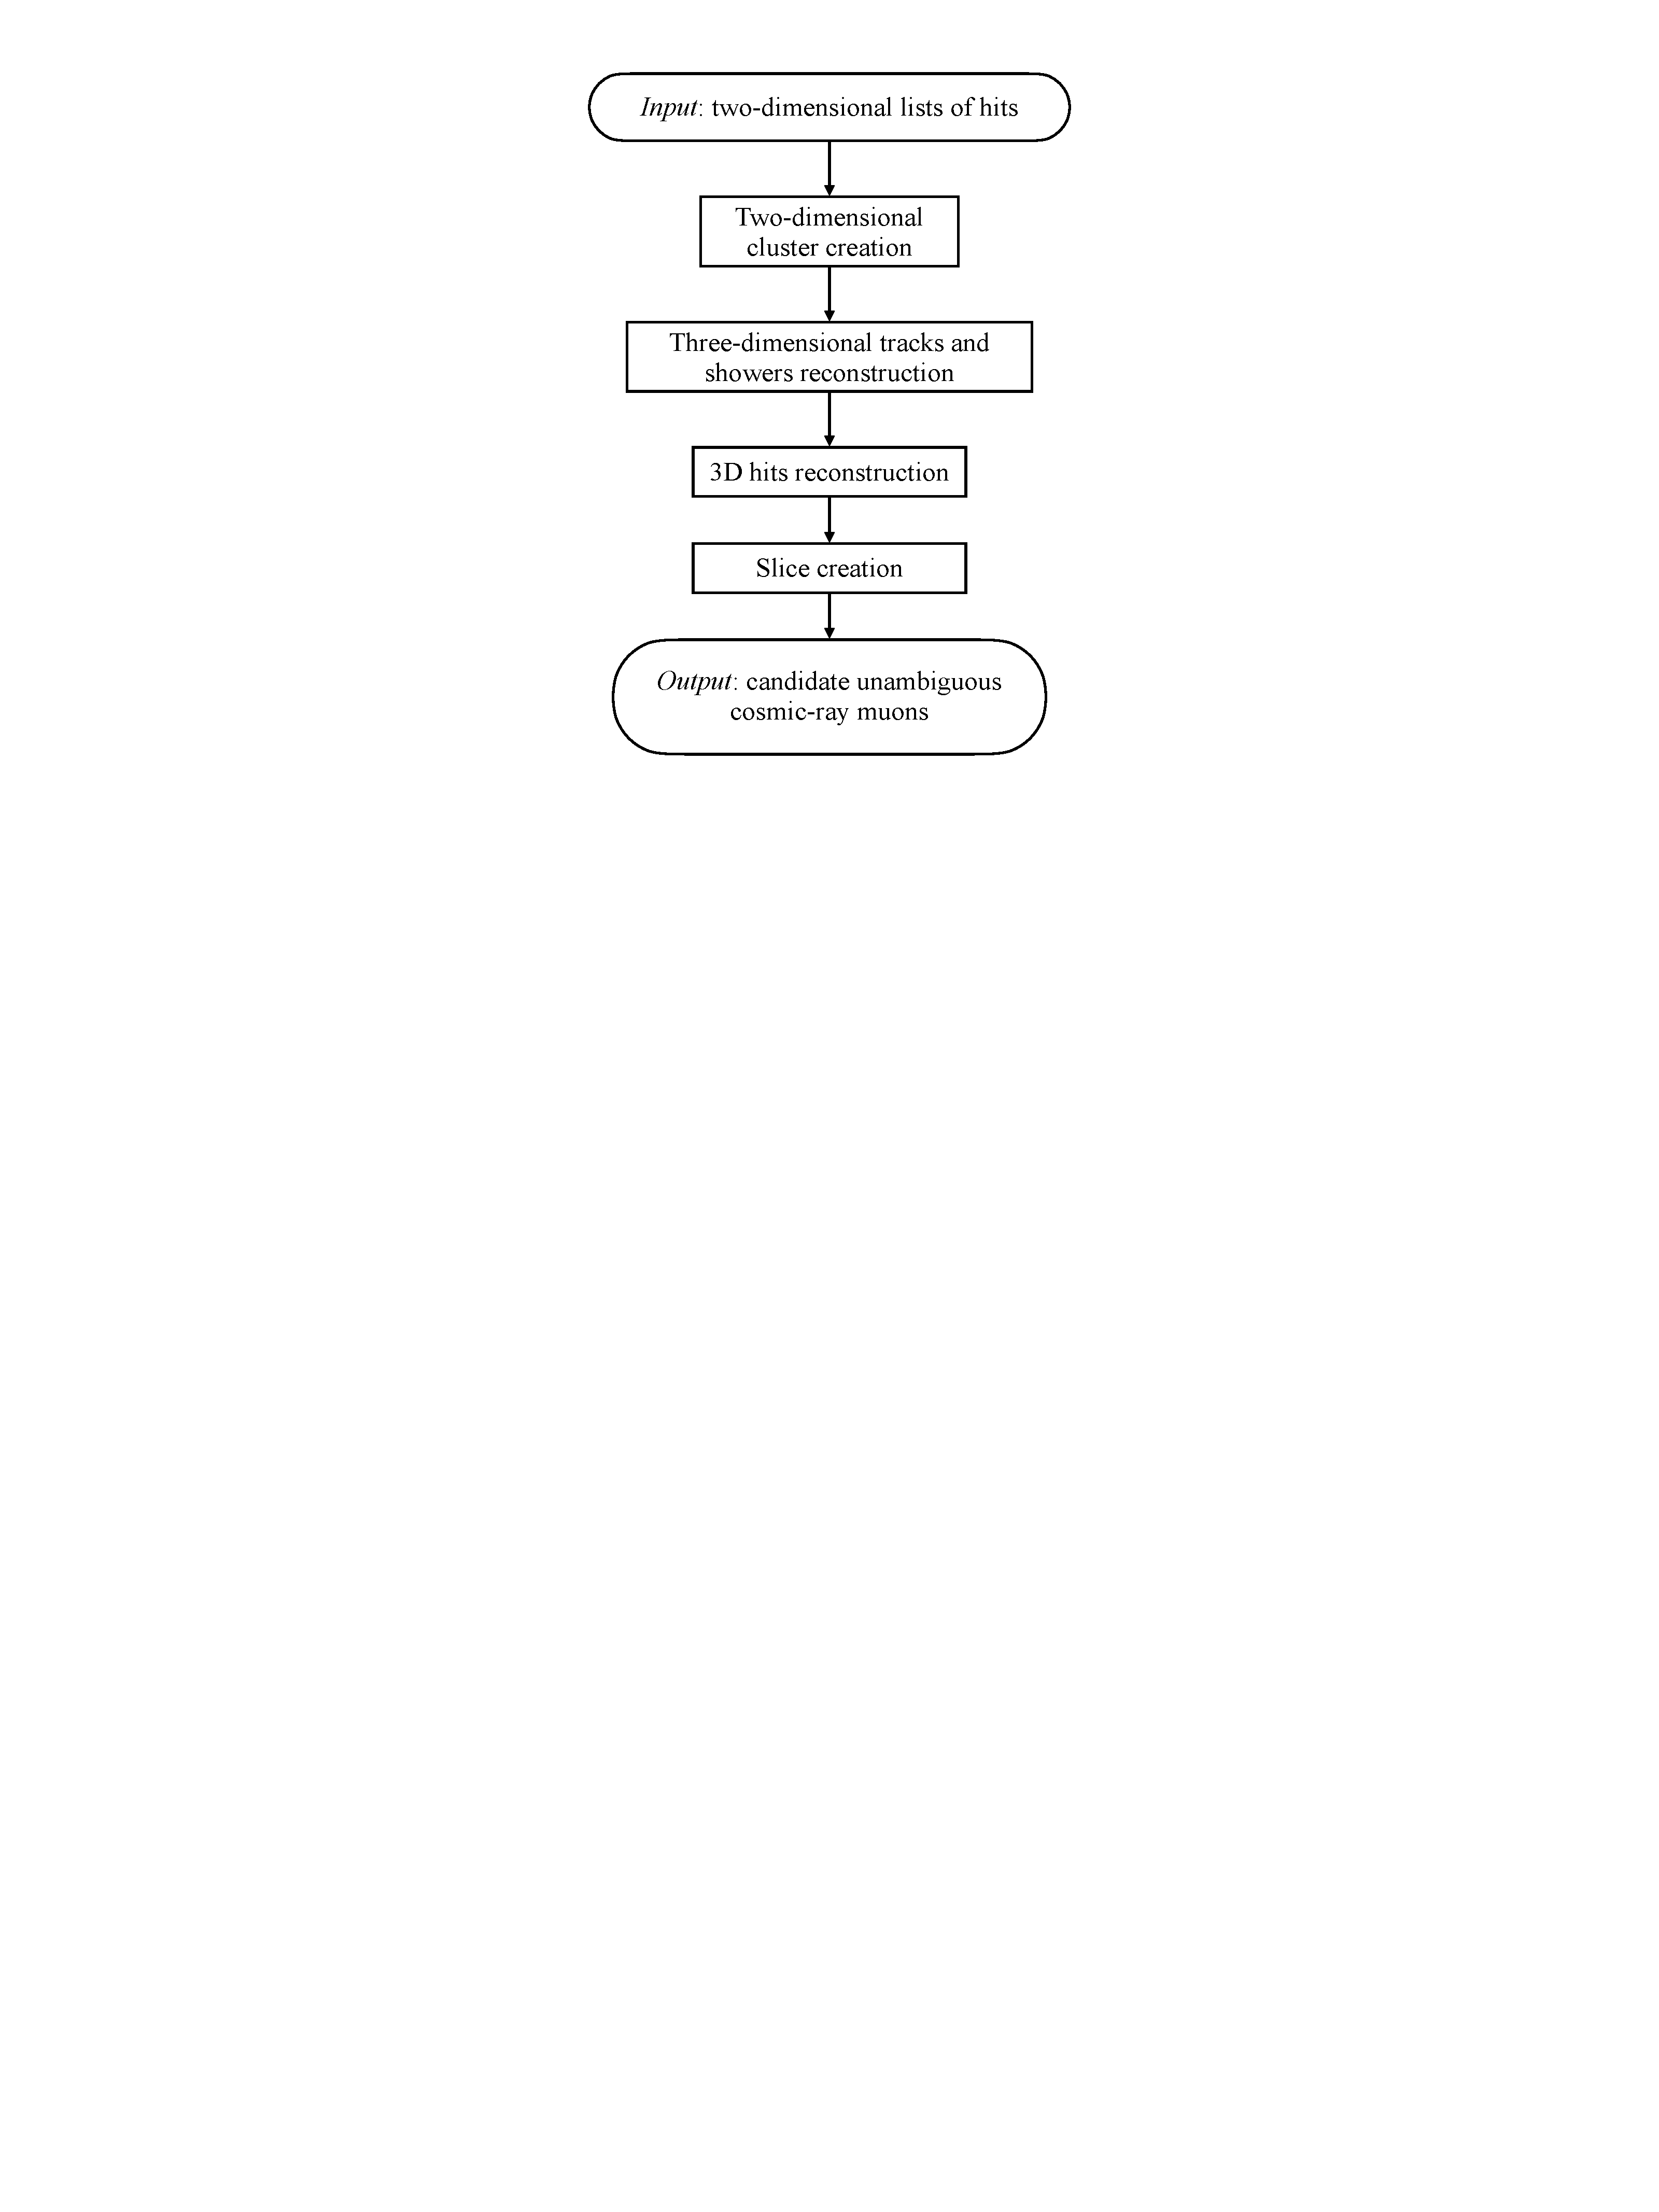
\includegraphics[width=0.5\linewidth,trim={16cm 47cm 16cm 1.5cm}, clip,page=1]{pandora/Pandora.pdf}
    \caption[PandoraFastReco path illustration]{Illustration of the main steps of the PandoraFastReco path, which is applied as a first coarse reconstruction. This path aims at creating unambiguous cosmic-ray muon candidates that are then flagged and whose hits are excluded from further processing. Figure adapted from \cite{MicroBooNE:2017xvs}}
    \label{fig:PandoraFastReco}
\end{figure}

\subsubsection{Two-dimensional reconstruction}

The first step takes as input the three separate lists of two-dimensional hits, corresponding to the three views or wire planes. For each, the TrackClusterCreation algorithm creates bidimensional clusters of hits, representing continuous lines of hits. Bifurcations, kinks or any topological branch-like feature stop the creation of a cluster and start the creation of another cluster. This approach ensures that clusters of hits created at this level have high purity, meaning a high number of correctly associated hits at the expense of completeness, meaning that a single true particle could be split into multiple clusters. At this point, cluster-merging algorithms identify associations between different 2D algorithms, improving the track completeness and affecting its purity in a minor way. Additionally, algorithms aimed at stitching together clusters that are split due to unresponsive wires or hits under the reconstruction threshold (that are not reconstructed) come into play at this level. 

To improve purity, cluster splitting algorithms refine the selection by breaking simple clusters if topological features indicate that there are ``spurious'' hits inside the cluster. 

\subsubsection{Three-dimensional reconstruction}

After 2D clusters are created, they are collected together with the aim of creating groups of 2D clusters that represent the same individual track particle. The challenge these algorithms need to address is to identify consistent groupings of clusters from the different views. The 3D track reconstruction is performed by three main algorithms: the ThreeDTransverseTracks algorithm, the ThreeDLongitudinalTracks algorithm and the ThreeDTrackFragments. The former algorithm has the biggest impact on three-dimensional track reconstruction.

The ThreeDTransverseTracks algorithm identifies all the suitable combinations of clusters from the three readout planes and inspects these combinations to identify cluster-matching ambiguities. These ambiguities are then used to improve the 2D cluster iteratively and remove them. The groupings of three clusters from the three readout planes are created by exploiting the common $x$ drift coordinate. On each view sliding fits are performed on the clusters; given a point on the $x$ coordinate, then the position of the sliding fit on two of the three views can be extracted, for example, the position on the $u$ and $v$ views. These positions, together with the coordinate transformation plugin, can be used to predict the position of the third cluster --- in the example shown in \autoref{fig:PandoraThreeDTracks}, in the $w$ view --- at the same $x$ drift coordinate. This prediction can be compared to the sliding fit position on the third view, and the same can be done with all possible combinations --- $u,v\to w$; $v,w\to u$ and $w, u \to v$. By performing such fits, and therefore checking the possible groupings of clusters across the three views, connections between them are created. The goal is to make these connections unambiguous, i.e. no two unique clusters from the same view are associated to the same unique cluster on another view. As described in \cite{MicroBooNE:2017xvs}, multiple tools query the different connection types across the views. Once no ambiguities are observed in the sets of clusters, the algorithm passes a list of sets of two (or three) clusters from different views to the following algorithms. Two examples showing how these tools operate on the 2D clusters are shown in \autoref{fig:PandoraThreeDTracks}. 

\begin{figure}
    \centering
    \subfloat[]{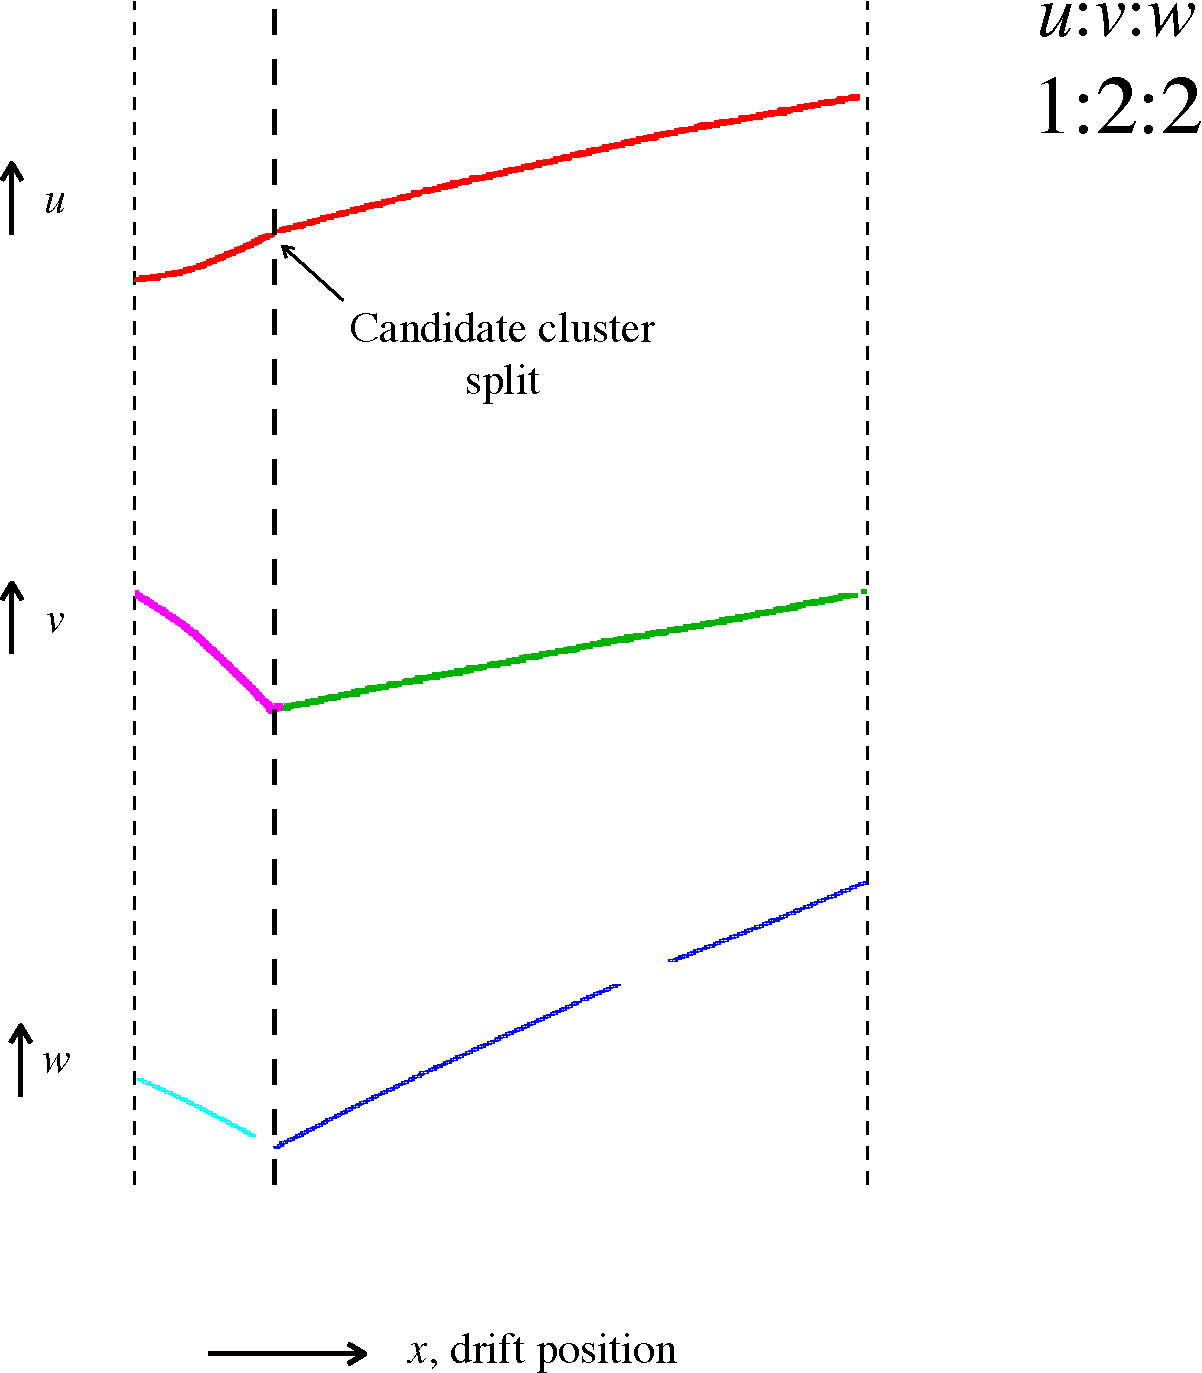
\includegraphics[width=0.5\linewidth]{pandora/ThreeDTracksTools/OvershootTracksTool.pdf}\label{fig:OvershootTracksTool}}
    \subfloat[]{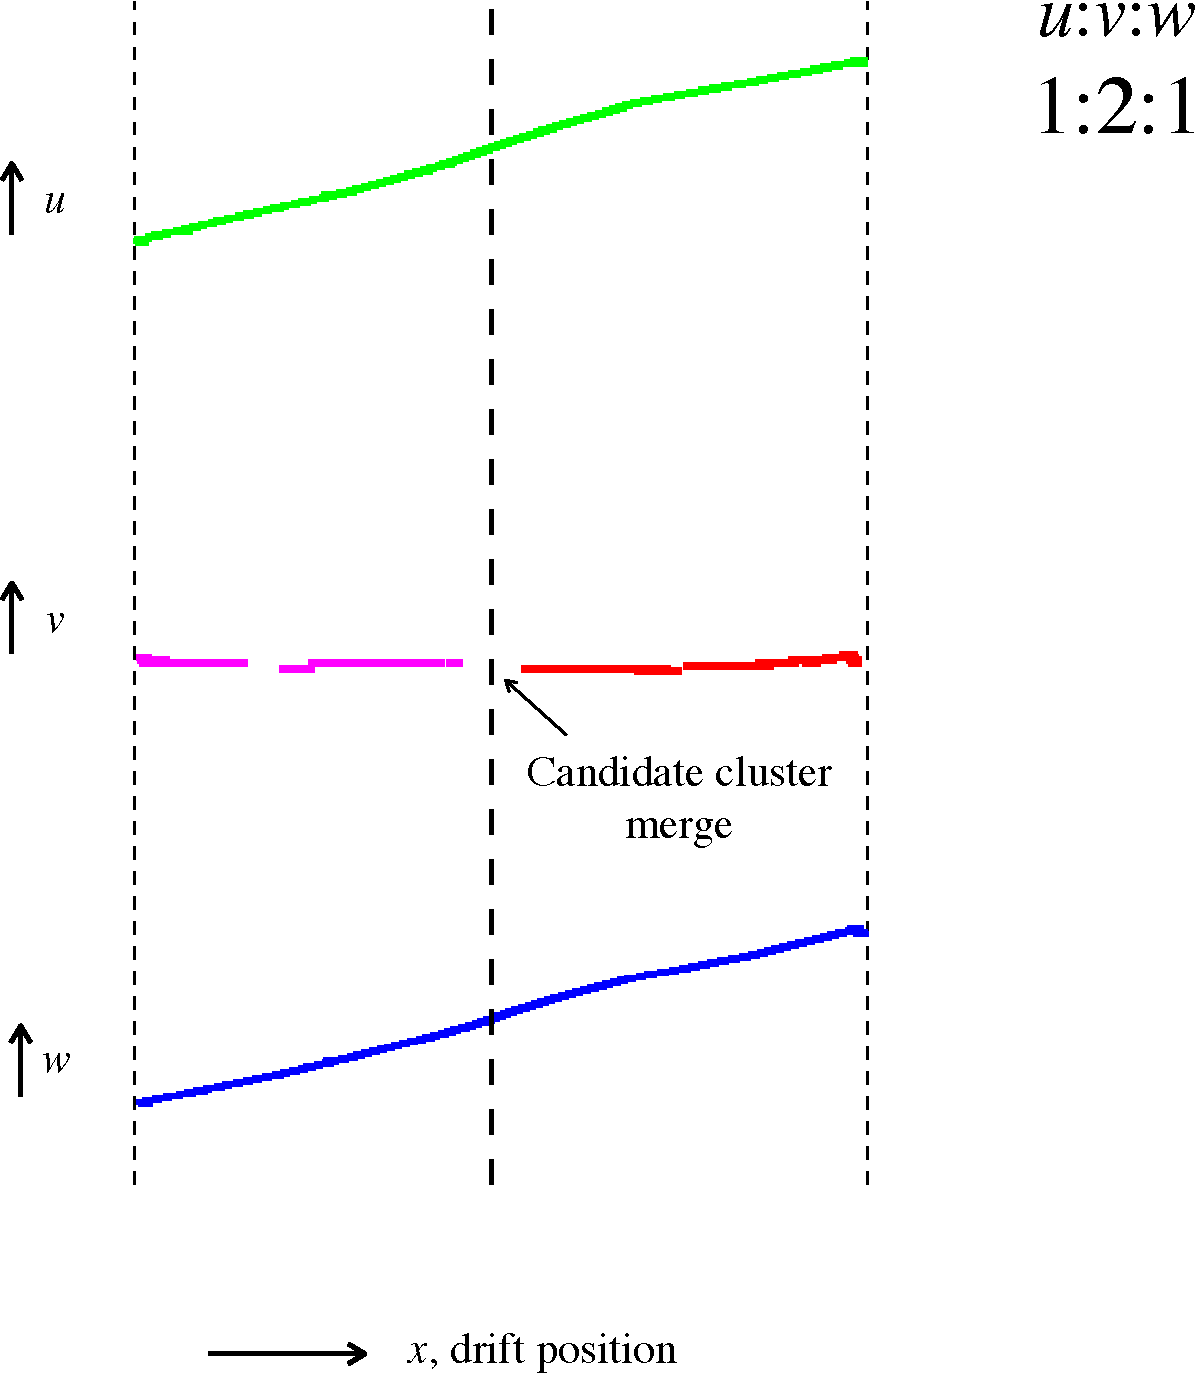
\includegraphics[width=0.5\linewidth]{pandora/ThreeDTracksTools/UndershootTracksTool.pdf}\label{fig:UndershootTracksTool}}
    \caption[Three-dimensional reconstruction helper tools]{Example of two of the tools querying the 2D clusters' connections. \ref{sub@fig:OvershootTracksTool} aims at resolving the ambiguities that arise from one view having two clusters merged into one. This ambiguity is resolved by splitting the cluster with the information from the other two views. \ref{sub@fig:UndershootTracksTool} has the opposite role and has the goal of merging cluster erroneously split into multiple pieces at previous stages. }
    \label{fig:PandoraThreeDTracks}
\end{figure}

\subsubsection{Three-dimensional hit reconstruction}

At this point, the assignment of hits to reconstructed particles is complete, each particle containing hits from two or usually three views. For each 2D hit a 3D point is created, with multiple approaches depending on the cluster topology. In all cases, the common step is the minimisation of a $\chi^2$-like value to get the best $y,z$ values for a given $x$ coordinate. 

After the 3D hit creation, candidate muon cosmic-ray particles are created, and they are tagged to filter out hits belonging to the unambiguously cosmic-ray particles. The remaining filtered hits are passed to subsequent paths of the reconstruction, namely PandoraCosmic and PandoraNeutrino. 

\subsection{PandoraNeutrino: topological neutrino event reconstruction} \label{sec:PandoraNeutrino}

A key requirement for the PandoraNeutrino reconstruction path is that it should be able to deal with the presence of cosmic-ray muon remnants. The approach to address this problem is therefore to run the same 2D clustering, 3D cluster matching and 3D hit reconstruction described in \autoref{sec:fast_reco}. After this path is run, 3D hits are divided into \emph{slices}, which are separate lists of clusters of lists, using proximity-based metrics. For a given event, the idea is to isolate the candidate neutrino interaction from any leftover cosmic-ray induced-tracks. The original 2D hits associated with each slice are then used as an input to the dedicated neutrino reconstruction, which is described in this section. 

The PandoraNeutrino dedicated reconstruction (shown in its entirety in Figure \ref{fig:PandoraNeutrino}) begins with a track-oriented clustering algorithm and a series of topological algorithms. Before processing the 2D clusters, the interaction vertex is reconstructed. 

\begin{figure}
    \centering
    \subfloat[]{\includegraphics[width=0.5\linewidth,trim={16cm 41cm 16cm 1.5cm}, clip,page=2]{pandora/Pandora.pdf}\label{fig:PandoraCosmic}}
    \subfloat[]{\includegraphics[width=0.5\linewidth,trim={16cm 40cm 16cm 1.5cm}, clip,page=3]{pandora/Pandora.pdf}\label{fig:PandoraNeutrino}}
    \caption[PandoraCosmic and PandoraNeutrino paths illustration]{\ref{sub@fig:PandoraCosmic} illustrates the PandoraCosmic path, applied after the first fast reco pass, in parallel with the neutrino path. \ref{sub@fig:PandoraNeutrino} illustration of the PandoraNeutrino reconstruction steps, applied to each slice in the event not tagged as cosmic induced interaction. Figure adapted from \cite{MicroBooNE:2017xvs}}
    \label{fig:PandoraCosmicNeutrino}
\end{figure}

\subsubsection{Three-dimensional vertex reconstruction}

The reconstruction of the neutrino interaction vertex proceeds via two steps. Firstly, the CandidateVertexCreation algorithm creates a list of possible vertices. Comparing pairs of 2D clusters and ensuring that they belong to different views and have a certain overlap as far as $x$ coordinate is concerned, the algorithm creates up to four neutrino vertex candidates for each 2D clusters pair, one for each endpoint of the 2D clusters. 

After the identification of the candidate neutrino vertices, it is necessary to identify the most probable vertex candidate. This step is achieved by means of a BDT algorithm, which assigns each vertex a score. The vertex candidate with the highest score is finally selected as the correct neutrino interaction vertex. 

The variables used to perform the classification and identify the most suitable vertex candidate include both properties of the reconstructed event and features of the candidate vertices. The former variables include the total number of hits, clusters and vertex candidates associated to the event, the fraction of hits likely originating from an electromagnetic shower based on cluster length and true associated particle, an estimate of the energy and of the 2D extent of the event, extracted from the total clusters span along $x$ and $z$ directions and an estimate of how longitudinal the event is with respect to the beam direction. 

This is the first of the three stages where Machine Learning techniques are employed within Pandora-based event reconstruction. 

\subsubsection{Three-dimensional track and shower reconstruction}

The PandoraNeutrino reconstruction, after the vertex creation stage, proceeds to reconstruct the three-dimensional tracks in the same way as described in previous sections. PandoraNeutrino, however, attempts also to reconstruct primary electromagnetic showers, arising from electrons and photons interacting in LAr. 

Using a set of topological cuts, 2D clusters are first classified either as track-like or shower-like. Existing track particles that are now deemed to be shower-like are dissolved, to allow assessment of the cluster as a shower candidate. At this point, on each view clusters representing shower branches candidates are merged. Showers are grown from the candidate shower spines adding shower branches where association is plausible. 

Following the 2D shower reconstruction, the ThreeDShowers algorithm builds the 3D hits in a similar way as for track-like particles. 

After the 3D showers are finally built, a second pass of the 3D track reconstruction is applied to recover any inefficiencies associated with dissolving track particles to examine their potential as showers. Once both 3D tracks and 3D showers are consolidated, particle refinement algorithms try to improve on both hit completeness and purity, dissolving unassociated 2D clusters or, especially in the case of showers, adding 2D clusters that were left from previous steps of the reconstruction. 

\subsubsection{Particle hierarchy reconstruction}

After the 3D reconstruction, the next step in the PandoraNeutrino reconstruction is to organise the reconstructed particles into a hierarchy. This follows some subsequent steps, namely \begin{itemize}
    \item An object associated to the neutrino particle is created and associated with the 3D interaction vertex.
    \item The 3D reconstructed particles deemed to be associated with the interaction vertex are added as primary daughters of the neutrino particle.
    \item Further event ramification takes place by associating secondary particles (if any) to the existing primary daughters of the neutrino, e.g. a decay electron could be associated to a primary muon particle decaying in the active detector volume.
    \item 3D vertex position and particle trajectory endpoints are calculated for each of the particles in the neutrino hierarchy. This is the neutrino interaction vertex for primary particles, and the point of closest approach to their parents for secondaries
\end{itemize}

The last step of the PandoraNeutrino reconstruction handles the classification, by means of a BDT algorithm, of reconstructed particles as tracks or showers. The classification is performed relying on a set of topological and calorimetric variables. A detailed description of the variables, the training process and the classification efficiency is discussed in \autoref{chap:mva_internship}, as part of the work performed during an internship at Fermilab. 

\subsection{PandoraCosmic: cosmic-ray muon reconstruction}

In parallel with to the neutrino-interaction reconstruction path, PandoraNeutrino, the PandoraCosmic path is also run, on the same set of hits, with the precise aim to reconstruct the remaining cosmic-ray interactions with greater detail compared to previous steps of the chain. 

The PandoraCosmic path is very similar to the PandoraFastReco path since it aims as well at the reconstruction of clear cosmic-ray muon particles. The only differences are the lack of the slice creation step, unique to the PandoraFastReco path, and the addition of the delta-ray reconstruction stage. This specific reconstruction path is illustrated in Figure \ref{fig:PandoraCosmic}. 

\subsubsection{Delta-ray reconstruction}

Unique to the PandoraCosmic path, before actually performing the creation of the 3D position inside the detector volume (see, for reference, Figure \ref{fig:PandoraCosmic}), a delta-ray reconstruction step deals with any 2D clusters that have not been assigned to any reconstructed particle. The assumption for these algorithms is that these clusters likely represent fragments of delta-ray showers. The hits leftover from previous reconstruction steps are reclustered and the between-views match is performed primarily exploiting the common $x$ coordinate. Parent cosmic ray particles are identified via comparisons of intra-cluster distances. 

\section{Calorimetry and particle identification} 

Following the topological event reconstruction performed by Pandora's set of algorithms, calorimetric information is computed with the use of multiple LArSoft modules. 

Once 3D trajectories, made of 3D space-points, have been reconstructed, using the relevant quantities associated with the hits --- hit area, hit time, and the track pitch lenght --- the target is reconstructing the energy loss as a function of residual range, i.e. $\dv*{E}{x}$, which is core to the  subsequent particle identification. The energy loss is computed for each hit from the $\dv*{Q}{x}$, expressed in ADC counts per centimeter. This in turn is obtained from the ratio of the area under the hit ($\dd Q$) and the track pitch ($\dd x$).  The latter is computed using the direction of the track taking into account that that the wire pitch for the ICARUS detector is of \SI{3}{\mm} and thus $\dd x = \SI{3}{\mm}/\cos\gamma$, where $\gamma$ is the three-dimensional angle between the local direction of the track and the wire direction. 

Calorimetry measurements require an accurate understanding of the charge response of the wires inside a LArTPC. The $\dv*{Q}{x}$ measured on the wires might substantially differ from the original $\dv*{Q}{x}$ at the location where the ionisation occurred; hence, it needs to be corrected before charge deposition is converted into energy loss. The process consisting in removing these charge response effects takes the name of ``charge equalisation''. This process is done in three separate steps: \begin{enumerate}
    \item charge equalisation in the drift direction $x$;
    \item the equalisation on the wireplane direction $y$ and $z$; and 
    \item the equalisation across the four TPCs in the ICARUS detector. 
\end{enumerate} Charge equalisation is performed using a dataset containing cosmic rays from off-beam events with muons crossing the LAr volume and leaving a signal in the CRT system.

The main effects that affect the $\dv*{Q}{x}$ in the ICARUS detector are \begin{itemize}
    \item Argon impurities: when electrons drift toward the anode, they can be captured by the electronegative impurities (mainly $\mathrm{O_2}$ and $\mathrm{H_2O}$). Since the electron attachment is modeled as an exponential decay, the measured $\dv*{Q}{x}$ is corrected as \begin{equation}
        \eval{\dv{Q}{x}}_\mathrm{corrected} = \eval{\dv{Q}{x}}_\mathrm{measured} \exp(\frac{t_\mathrm{hit}-t_0}{\tau}),
    \end{equation} where $\tau$ is the electron lifetime. The electron lifetime measured in the ICARUS detector in a range between 4 and \SI{8}{\ms}. For the second ICARUS data taking run, the electron lifetime was measured to be ${\sim}\SI{4}{\ms}$ for the East and ${\sim}\SI{7}{\ms}$ for the West cryostat. 

    \item Drift field distortions: the ionisation process inside liquid argon, other than producing a plethora of free electrons, gives rise to Ar ions. They in turn contribute to to disuniformities of the drift electric field. Additionally, the ICARUS cathode plane is not completely flat, and this also produces disuniformities of the field. Absolute variations were found to vary from \qtyrange{-6}{13}{\mm} in the East cryostat, while West cryostat reported values between \SI{+-9}{\mm} \cite{arteroponsStudyReconstructionNuMuCC}. This impacts the electric field uniformity and results in a difference of the drift time of about ${\sim}\SI{8}{\us}$. 

    \item Diffusion: electrons do not drift following perfectly linear trajectories to the anodes but get diffused by elastic interaction in LAr. 
\end{itemize} Details on the countermeasures adopted to account for such effects are provided in \cite{arteroponsStudyReconstructionNuMuCC}. 

As part of the calibrations steps, to convert the $\dv*{Q}{x}$ into a deposited energy value, we need to take into account the fraction of electrons that survive the recombination process, $\mathcal{R}$, the amount of energy that is required to ionise an argon atom, $W_\mathrm{ion} = \SI{23.6}{eV}$ \cite{navasReviewParticlePhysics2024} and the electronic gain $\mathcal{G}$ that converts ADC counts into the number of drifted electrons collected on the readout planes. With these details, it is possible to compute the $\dv*{E}{x}$ like \begin{equation}
    \dv{E}{x} = \frac{W_\mathrm{ion}}{\mathcal{R\cdot G}} \dv{Q}{x}. 
\end{equation}

From the reconstructed energy deposition per centimeter, it is possible to compute the full deposited energy like \begin{equation}
    E = \sum_i^\mathrm{all\ hits} \qty(\dv{E}{x} )_i \cdot \dd x_i. 
\end{equation}

Using the calorimetric information, it is possible to develop a $\chi^2$-like score that helps us identify the particle species. The underlying assumption is that, if the particle stops inside the TPC active volume, the $\dv*{E}{x}$ energy loss versus the residual range\footnote{Residual range is defined as the distance of an energy deposition within a track from the track's endpoint.} is a means to distinguish charged particles. In the $\chi^2$ score definition, the measured $\dv*{E}{x}$ for a given reconstructed track is compared, on a hit basis, with the average response predicted under different particle hypotheses from the Bethe formula, including protons, charged kaons, charged pions and muons as viable options. The PID score is defined as this value, divided by the number of hits in the track \cite{arteroponsStudyReconstructionNuMuCC} \begin{equation}
    \mathrm{PID} = \chi^2/\mathrm{ndof} = \sum_\mathrm{hit} \qty(\frac{{\dv*{E}{x}}_\mathrm{measured} - {\dv*{E}{x}}_\mathrm{theory}}{\sigma_{\dv*{E}{x}}})^2 \Big/ n_\mathrm{hits}. \label{eq:PID}
\end{equation} where $\sigma_{\dv*{E}{x}}$ is an estimate of the resolution on the measured $\dv*{E}{x}$ per hit (${\sim}\SI{3}{\percent}$) and was evaluated in dedicated studies by ArgoNeuT \cite{ArgoNeuT:2013kpa}.

\section{SPINE: machine learning particle identification} \label{sec:SPINE}

Inside the ICARUS collaboration, an effort to develop an ML-based end-to-end reconstruction chain started and has now reached a mature stage, at which the performances and the robustness of the tools allow for analyses to be performed. This approach, named SPINE (Scalable Particle Imaging with Neural Embedding) \cite{Drielsma:2021jdv}, consists of a hierarchical set of neural networks that are part of an optimisible end-to-end reconstruction chain.

A schematic representation of the SPINE sequence is shown in \autoref{fig:SPINE}. 

The starting point for the reconstruction are the three-dimensional space points processed by the Cluster3D algorithm. The hits that come out of the Cluster3D algorithm are passed through a UResNet architecture that aims at removing the so-called ghost hits. These are 3D hits resulting from an incorrect combination of 2D hits. Filtered positions are referred to as ``deghosted'' 3D space points. 

\begin{figure}
    \centering
    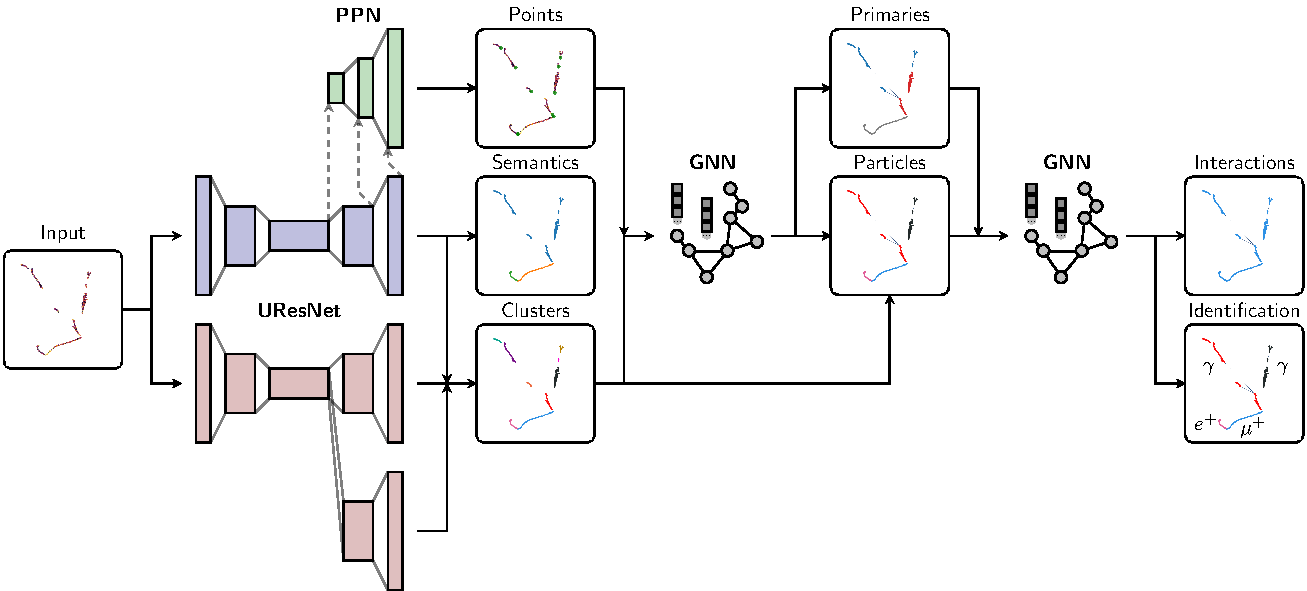
\includegraphics[width=\linewidth]{detector/mlreco_full_chain.pdf}
    \caption[SPINE end-to-end machine learning approach]{Schematic architecture of the end-to-end, ML-based reconstruction chain for LArTPCs. Picture taken from \cite{Drielsma:2021jdv}. }
    \label{fig:SPINE}
\end{figure}

The next step in the reconstruction chain is the classification of the deghosted 3D hits into categories based on the activity that produced them --- tracks, electromagnetic showers, Michel electrons, delta rays and low-energy depositions. This algorithm (shown in blue in \autoref{fig:SPINE}) uses the same UResNet architecture as the previous step. In parallel with this (shown in red in \autoref{fig:SPINE}) is a similar algorithm that aims at identifying and building dense particle clusters. The two outputs are aggregated and then passed as input to the next steps of the reconstruction. 


At this point of the SPINE reconstruction chain, groups of spacepoints corresponding to particle fragments have been identified, with semantic labels assigned to them. Then, a Graph Neural Network (GNN) aims at clustering these groups of hits into particles. Two functionally identical GNNs are employed, called GrapPA-Track and GrapPA-Shower, targeting specific interaction topologies, namely tracks and showers. Details on the implementation and working principle of these algorithms are given in \cite{Drielsma:2021jdv}. 

The final stage of the SPINE reconstruction is to cluster particles into interactions. A given interaction (equivalent to a Pandora slice) is a collection of particles originating from the same interaction vertex. Particles directly associated with the interaction vertex are called primary particles, whereas other particles are labelled as secondaries. In addition to the interaction clustering, the network is also tasked with predicting the particle type (photon, electron, muon, proton, or pion; see \cite{DeepLearnPhysics:2020hut}). The architecture is still that of a GNN. The output of this network is represented by all the interaction primary particles, each with a list of secondary particles, all with their types. 

\section{Simulation of the full detector}

\begin{figure}
    \centering
    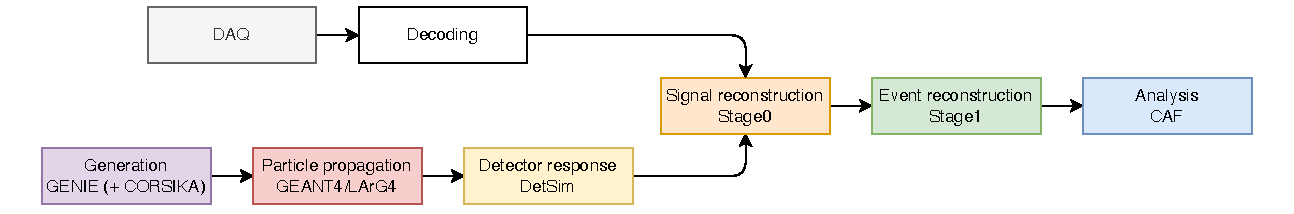
\includegraphics[width=\linewidth]{pandora/LArSoft_all.drawio.pdf}
    \caption[LArSoft complete overview]{Complete processing flow for both data and simulation, from the collection/simulation to the final analysis. }
    \label{fig:LArSoft_flow}
\end{figure}

The LArSoft framework that runs the full event reconstruction is also used to perform event simulation, from the generation of the interaction, performed using the GENIE Monte Carlo neutrino generator \cite{Andreopoulos:2015wxa}, to  particle propagation inside the LAr volume, performed using the GEANT4 package, accessed through the LArG4 framework, to detector simulation, covering all the individual subsystems of the ICARUS detector. The output of the simulation is identical to the real acquired data collected by the detector and therefore can be used to perform Monte Carlo studies on the reconstruction pipeline. Details of the full event simulation are in \cite{arteroponsStudyReconstructionNuMuCC}, and \autoref{fig:LArSoft_flow} shows a full overview of the entire pipeline both for real data, starting from the DAQ (above), to decoding and then signal processing and event reconstruction, as well as for simulated data (below).